\chapter{METODOLOGI PENELITIAN}

Penelitian ini membandingkan \textit{Mixture of Inputs} (MoI), yaitu
metode \textit{reasoning} melalui representasi laten, dengan tiga metode
lain: \code{raw} (\textit{input-output alignment}), \code{soft}
(\textit{Soft Thinking}), dan \code{sample} (\textit{discrete token}). Keempatnya
diterapkan pada sistem multi-agen yang berkomunikasi melalui transfer
\textit{KV-cache}, yang selanjutnya juga dibandingkan dengan sistem
multi-agen standar berbasis teks.

%==========================================================================
\section{Arsitektur Qwen3-8B}

\label{sec:m-arsitektur}

Qwen3-8B merupakan model bahasa autoregresif dengan arsitektur
\textit{Transformer decoder-only} \citep{qwen3} dengan
\textit{hidden layer} $L=36$ lapisan dan dimensi \textit{hidden state} $d=4096$.

Gambar~\ref{fig:m-latent-overview} memperlihatkan alur komputasi yang
digunakan sebagai dasar pembahasan. Teks \textit{input} diubah menjadi token(\textit{tokenization}), 
kemudian dipetakan melalui \textit{embedding} masukan $W_{\mathrm{in}}$ menjadi vektor.
Hasil \textit{embedding} tersebut diproses melalui seluruh blok \textit{decoder} 
hingga menghasilkan \textit{hidden state} $h_k$. \textit{Hidden state} dipetakan melalui \textit{output projection} $W_{\mathrm{out}}$ 
menjadi \textit{logit}, yang kemudian diubah menjadi \textit{probability} melalui fungsi \textit{softmax}.
Probabilitas digunakan untuk menghitung bobot $w_k$ yang digunakan untuk membentuk representasi laten $\tilde{z}_k$.
Representasi laten tersebut kemudian dinormalisasi menjadi $z_k$ sebelum dikembalikan ke \textit{embedding} masukan untuk langkah berikutnya.

\begin{figure}[H]
\centering
\begin{tikzpicture}[
node distance=7mm,
box/.style={
draw,
rounded corners,
align=center,
minimum width=4.0cm,
minimum height=8mm
},
smallbox/.style={
draw,
rounded corners,
align=center,
minimum width=3.4cm,
minimum height=8mm
},
arrow/.style={->, >=stealth}
]
    \node[box] (token) {Token\\$x_t$};
    \node[box, below=of token] (embed)
    {\textit{Embedding} masukan\\$W_{\mathrm{in}}[x_t]$};
    \node[box, below=of embed] (decoder)
    {Blok \textit{decoder}\\$\times L$};
    \node[box, below=of decoder] (hidden)
    {\textit{Hidden state}\\$h_k$};

    \node[smallbox, below left=10mm and 2mm of hidden] (raw)
        {\code{raw}\\$\tilde{z}_k=h_kM$};

    \node[smallbox, below right=10mm and 2mm of hidden] (logit)
        {\textit{Logit}\\$\ell_k=W_{\mathrm{out}}h_k$};

    \node[smallbox, below=of logit] (prob)
        {\textit{Probability}\\$p_k=\operatorname{softmax}(\ell_k/T)$};

    \node[smallbox, below=of prob] (weight)
        {Bobot $w_k$\\\code{soft}, \code{sample}, \code{moi}};

    \node[box, below=29mm of raw] (latent)
        {Representasi laten\\$\tilde{z}_k$};

    \node[box, below=of latent] (normal)
        {Normalisasi \\$z_k=\tau\tilde{z}_k/\|\tilde{z}_k\|_2$};

    \draw[arrow] (token) -- (embed);
    \draw[arrow] (embed) -- (decoder);
    \draw[arrow] (decoder) -- (hidden);

    \draw[arrow] (hidden) -- (raw);
    \draw[arrow] (hidden) -- (logit);
    \draw[arrow] (logit) -- (prob);
    \draw[arrow] (prob) -- (weight);

    \draw[arrow] (raw) -- (latent);
    \draw[arrow] (weight) -- (latent);

    \draw[arrow] (latent) -- (normal);
    \draw[arrow] (normal.south) -- ++(0, -6mm)
        -- ++(-35mm, 0)
        |- (embed.west);
\end{tikzpicture}
\caption{Alur representasi laten pada arsitektur Qwen3.}
\label{fig:m-latent-overview}

\end{figure}


\subsection{Blok \textit{Decoder}}
\label{subsec:m-decoder}

Masukan bagi lapisan pertama blok \textit{decoder} adalah barisan
vektor \textit{embedding} token. Jika $x_t\in\{1,\ldots,V\}$
menyatakan indeks token pada posisi $t$, maka representasi awal
token tersebut dapat dituliskan sebagai
\begin{equation}
x_t^{(0)}=W_{\mathrm{in}}[x_t],
\label{eq:m-arch-input}
\end{equation}

dengan $W_{\mathrm{in}}\in\mathbb{R}^{V\times d}$
dan $x_t^{(0)}\in\mathbb{R}^{d}$.

Setiap lapisan(\textit{layer}) ke-$l$, untuk $l=1,\ldots,L$, terdiri atas dua
sublapisan, yaitu mekanisme atensi (\textit{attention}) yang
menggabungkan informasi antarposisi dan jaringan umpan-maju
(\textit{feed-forward network}).
Transformasi pada posisi $t$ dapat dituliskan sebagai

\begin{align}
\widetilde{x}_t^{(l)}
&=
x_t^{(l-1)}
+
\operatorname{Attn}^{(l)}
\left(
\operatorname{RMSNorm}
\left(x_t^{(l-1)}\right)
\mid
\mathrm{KV}_{1:t}^{(l)}
\right),
\label{eq:m-arch-attn}
\\[2pt]
x_t^{(l)}
&=
\widetilde{x}_t^{(l)}
+
\operatorname{MLP}^{(l)}
\left(
\operatorname{RMSNorm}
\left(\widetilde{x}_t^{(l)}\right)
\right),
\label{eq:m-arch-mlp}
\end{align}

dengan $x_t^{(l-1)},\widetilde{x}_t^{(l)},x_t^{(l)}
\in\mathbb{R}^{d}$ menyatakan representasi token
pada tahapan yang berbeda. Notasi
$\mathrm{KV}_{1:t}^{(l)}$ menyatakan kumpulan representasi
\textit{key} dan \textit{value} internal pada lapisan ke-$l$
untuk posisi $1,\ldots,t$. Simbol $\mid$ memisahkan masukan
\textit{query} dari kumpulan \textit{key} dan \textit{value}
yang digunakan dalam perhitungan atensi.

Setelah seluruh $L$ lapisan selesai diproses, representasi pada
posisi terakhir dinormalisasi kembali untuk memperoleh
\textit{hidden state} yang digunakan oleh metode laten. Jika
posisi terakhir dinyatakan dengan indeks $T$, maka
\begin{equation}
h_T
=
\operatorname{RMSNorm}\left(x_T^{(L)}\right),
\qquad
h_T\in\mathbb{R}^{d}.
\label{eq:m-arch-h}
\end{equation}

Normalisasi yang digunakan adalah
\textit{Root Mean Square Normalization} (RMSNorm). Untuk suatu
vektor $x\in\mathbb{R}^{d}$, RMSNorm didefinisikan sebagai
\begin{equation}
\operatorname{RMSNorm}(x)
=
\frac{x}{
\sqrt{
\frac{1}{d}\sum_{j=1}^{d}x_j^2+\epsilon
}
}
\odot g,
\qquad
\epsilon=10^{-6},
\label{eq:m-arch-rmsnorm}
\end{equation}
dengan $g\in\mathbb{R}^{d}$ merupakan vektor parameter penguatan
yang dipelajari, $\epsilon$ merupakan konstanta untuk menjaga
stabilitas perhitungan, dan $\odot$ menyatakan perkalian Hadamard.
Dimensi $d$ menyesuaikan dimensi vektor yang dinormalisasi.

Sublapisan umpan-maju(\textit{feed-forward}) menggunakan struktur SwiGLU, yaitu varian
jaringan umpan-maju yang menggabungkan mekanisme gerbang
(\textit{gating}) dengan fungsi aktivasi SiLU. Untuk masukan
$x\in\mathbb{R}^{d}$, transformasinya
didefinisikan sebagai

\begin{equation}
\operatorname{MLP}(x)
=
W_{\mathrm{down}}
\left(
\operatorname{SiLU}(W_gx)
\odot
(W_{\mathrm{up}}x)
\right),
\label{eq:m-arch-swiglu}
\end{equation}

dengan
$W_g,W_{\mathrm{up}}
\in\mathbb{R}^{d_{\mathrm{ff}}\times d}$
merupakan matriks proyeksi dari dimensi model ke dimensi
tersembunyi, sedangkan
$W_{\mathrm{down}}
\in\mathbb{R}^{d\times d_{\mathrm{ff}}}$
merupakan matriks proyeksi kembali ke dimensi model.

Matriks $W_g$ memproyeksikan masukan ke jalur gerbang, sedangkan
$W_{\mathrm{up}}$ memproyeksikan masukan ke jalur informasi.
Keluaran kedua jalur digabungkan melalui perkalian Hadamard,
untuk diproyeksikan kembali melalui $W_{\mathrm{down}}$.

Fungsi SiLU didefinisikan sebagai
\begin{equation}
\operatorname{SiLU}(a)=a\,\sigma(a),
\label{eq:m-arch-silu}
\end{equation}

dengan $a\in\mathbb{R}$ dan
$\sigma(a)=1/(1+\exp(-a))$ merupakan fungsi sigmoid.
Untuk masukan berbentuk vektor, fungsi tersebut diterapkan
pada setiap komponennya secara terpisah.

\subsection{\textit{Grouped-Query Attention} dan RoPE}

\label{subsec:m-gqa}

Sub-lapisan \textit{attention} Qwen3-8B menggunakan \textit{grouped-query attention}
(GQA). Model memiliki $H_q=32$ \textit{query heads} dan
$H_{kv}=8$ pasangan \textit{key-value heads} \citep{qwen3}. Dengan
demikian, beberapa \textit{query heads} berbagi pasangan
\textit{key-value} yang sama.

Dimensi setiap \textit{head} ditentukan oleh

\begin{equation}
d_k
=
\frac{d}{H_q}
=
\frac{4096}{32}
=
128.
\label{eq:m-arch-dk}
\end{equation}

Untuk \textit{query head} ke-$\eta$, dengan
$\eta\in\{1,\ldots,32\}$, indeks pasangan \textit{key-value} yang
digunakan dapat dinyatakan sebagai

\begin{equation}
g(\eta)
=
\left\lceil
\frac{\eta}{H_q/H_{kv}}
\right\rceil
=
\left\lceil
\frac{\eta}{4}
\right\rceil,
\qquad
g(\eta)\in\{1,\ldots,8\}.
\label{eq:m-arch-gqa}
\end{equation}


\begin{figure}[H]
    \centering
    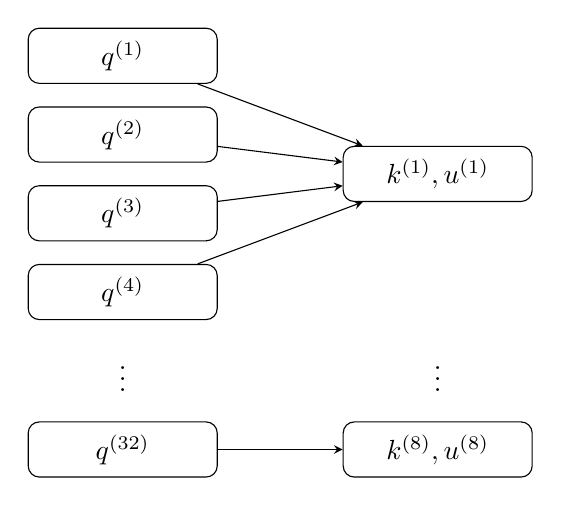
\begin{tikzpicture}[
        box/.style={
            draw,
            rounded corners,
            align=center,
            minimum width=2.4cm,
            minimum height=7mm
        },
        arrow/.style={->, >=stealth}
    ]
        \node[box] (q1) at (0,2.0) {$q^{(1)}$};
        \node[box] (q2) at (0,1.0) {$q^{(2)}$};
        \node[box] (q3) at (0,0.0) {$q^{(3)}$};
        \node[box] (q4) at (0,-1.0) {$q^{(4)}$};

        \node[box] (kv1) at (4,0.5)
            {$k^{(1)},u^{(1)}$};

        \draw[arrow] (q1) -- (kv1);
        \draw[arrow] (q2) -- (kv1);
        \draw[arrow] (q3) -- (kv1);
        \draw[arrow] (q4) -- (kv1);

        \node at (0,-2.0) {$\vdots$};
        \node at (4,-2.0) {$\vdots$};

        \node[box] (q32) at (0,-3.0) {$q^{(32)}$};
        \node[box] (kv8) at (4,-3.0)
            {$k^{(8)},u^{(8)}$};

        \draw[arrow] (q32) -- (kv8);
    \end{tikzpicture}
    \caption{Ilustrasi pembagian \textit{query heads} pada GQA.}
    \label{fig:m-gqa}
\end{figure}


Untuk \textit{query head} ke-$\eta$, \textit{query}, \textit{key}, dan \textit{value} diperoleh melalui proyeksi dari vektor masukan yang telah dinormalisasi, yaitu $x\in\mathbb{R}^{d}$, melalui

\begin{equation}
q^{(\eta)}
=
W_Q^{(\eta)}x,
\qquad
k^{(g(\eta))}
=
W_K^{(g(\eta))}x,
\qquad
v^{(g(\eta))}
=
W_V^{(g(\eta))}x,
\label{eq:m-arch-qku}
\end{equation}

dengan $W_Q^{(\eta)}$, $W_K^{(g(\eta))}$, $W_V^{(g(\eta))}\in\mathbb{R}^{d_k\times d}$
merupakan matriks proyeksi yang dipelajari selama pelatihan dan $q^{(\eta)},k^{(g(\eta))}$, 
$v^{(g(\eta))}\in\mathbb{R}^{d_k}$.

Sebelum digunakan dalam perhitungan \textit{attention}, informasi posisi direpresentasikan menggunakan \textit{Rotary Position Embedding} (RoPE) \citep{roformer}.


\begin{definisi}[Rotary Position Embedding (RoPE)]
\label{def:rope}
Rotary Position Embedding (RoPE) merupakan transformasi yang
merepresentasikan informasi posisi token melalui rotasi pasangan
komponen vektor. Untuk pasangan komponen ke-$r$ pada posisi $t$,
transformasi tersebut didefinisikan sebagai
\begin{equation}
\begin{pmatrix}
x'_{t,2r}\\
x'_{t,2r+1}
\end{pmatrix}
=
\begin{pmatrix}
\cos\theta_{t,r} & -\sin\theta_{t,r}\\
\sin\theta_{t,r} & \cos\theta_{t,r}
\end{pmatrix}
\begin{pmatrix}
x_{t,2r}\\
x_{t,2r+1}
\end{pmatrix},
\label{eq:m-arch-rope}
\end{equation}

dengan $x_{t,2r}$ dan $x_{t,2r+1}$ menyatakan dua komponen
vektor sebelum rotasi, $x'_{t,2r}$ dan $x'_{t,2r+1}$ menyatakan
komponen setelah rotasi, serta $\theta_{t,r}$ menyatakan sudut
rotasi yang bergantung pada posisi $t$ dan indeks pasangan $r$.
Transformasi ini diterapkan pada vektor \textit{query} dan
\textit{key} sebelum perhitungan \textit{attention}.
\end{definisi}

Berdasarkan Definisi~\ref{def:rope}, penerapan RoPE pada
\textit{query} di posisi $i$ dan \textit{key} di posisi $j$
dinyatakan sebagai

\begin{equation}
\begin{aligned}
\widetilde{q}_i^{(\eta)}
&=
\operatorname{RoPE}_i\left(q_i^{(\eta)}\right),\\
\widetilde{k}_j^{(g(\eta))}
&=
\operatorname{RoPE}_j\left(k_j^{(g(\eta))}\right).
\end{aligned}
\label{eq:m-arch-rope-qk}
\end{equation}

dengan $i,j\in\{1,\ldots,L\}$ masing-masing menyatakan posisi
\textit{query} dan \textit{key} dalam urutan sepanjang $L$ token,
serta $q_i^{(\eta)},\widetilde{q}_i^{(\eta)},
k_j^{(g(\eta))},\widetilde{k}_j^{(g(\eta))}
\in\mathbb{R}^{d_k}$ merupakan vektor \textit{query} dan
\textit{key} sebelum dan sesudah penerapan RoPE.

Vektor hasil rotasi tersebut digunakan untuk menghitung skor
kesesuaian antara \textit{query} dan \textit{key} yang dinormalisasi
untuk menghasilkan bobot \textit{attention}. Untuk posisi
\textit{query} $i$ dan posisi \textit{key} $j$, bobot
\textit{attention} dapat dituliskan sebagai
\begin{equation}
\begin{gathered}
\alpha_{ij}^{(\eta)}
=
\frac{
\exp\left(
\frac{
\left(\widetilde{q}_i^{(\eta)}\right)^{\mathsf T}
\widetilde{k}_j^{(g(\eta))}
}{
\sqrt{d_k}
}
\right)
}{
\displaystyle
\sum_{r=1}^{i}
\exp\left(
\frac{
\left(\widetilde{q}_i^{(\eta)}\right)^{\mathsf T}
\widetilde{k}_r^{(g(\eta))}
}{
\sqrt{d_k}
}
\right)
},
\\[6pt]
\alpha_{ij}^{(\eta)}\geq 0,
\qquad
\sum_{j=1}^{i}\alpha_{ij}^{(\eta)}=1.
\end{gathered}
\label{eq:m-arch-attention-weight}
\end{equation}
dengan $r$ merupakan indeks penjumlahan posisi \textit{key}
yang berjalan dari $1$ hingga $i$,
$\alpha_{ij}^{(\eta)}\in[0,1]$ merupakan bobot skalar
\textit{attention} antara \textit{query} pada posisi $i$
dan \textit{key} pada posisi $j$.

Bobot $\alpha_{ij}^{(\eta)}$ selanjutnya digunakan untuk
menggabungkan vektor \textit{value} pada posisi-posisi yang
dapat diakses oleh \textit{query}. Keluaran \textit{attention}
untuk \textit{query head} ke-$\eta$ pada posisi $i$ dapat
dituliskan sebagai
\begin{equation}
o_i^{(\eta)}
=
\sum_{j=1}^{i}
\alpha_{ij}^{(\eta)}
u_j^{(g(\eta))},
\qquad
o_i^{(\eta)}\in\mathbb{R}^{d_k}.
\label{eq:m-arch-attention-output}
\end{equation}
dengan $u_j^{(g(\eta))}\in\mathbb{R}^{d_k}$ merupakan vektor
\textit{value} pada posisi $j$ untuk \textit{key-value head}
ke-$g(\eta)$, sedangkan $o_i^{(\eta)}$ merupakan hasil
penjumlahan bobot \textit{attention} dengan vektor \textit{value}.

Persamaan tersebut memperlihatkan bahwa RoPE memengaruhi perhitungan
kesesuaian antara \textit{query} dan \textit{key}, sedangkan vektor
\textit{value} digunakan untuk membentuk keluaran \textit{attention}. Sehingga
\textit{KV-cache} dapat digunakan untuk mempertahankan informasi token
dari posisi-posisi sebelumnya.

\subsection{\textit{KV-cache} per Lapisan}

\label{subsec:m-kvcache}

Pada \textit{Transformer decoder-only}, hasil proyeksi \textit{key} dan
\textit{value} dari posisi-posisi sebelumnya dapat disimpan sehingga tidak
perlu dihitung ulang ketika posisi baru diproses. Penyimpanan tersebut
disebut \textit{KV-cache}.

Untuk lapisan ke-$l$, setelah $t$ posisi diproses,
\textit{KV-cache} secara konseptual dapat dituliskan sebagai

\begin{equation}
\mathrm{KV}^{(l)}_t
=
\left\{
\left(
k_j^{(l,g)},
v_j^{(l,g)}
\right)
:
1\leq j\leq t,\;
1\leq g\leq H_{kv}
\right\}.
\label{eq:m-arch-kv}
\end{equation}

Karena Qwen3-8B memiliki $H_{kv}=8$, setiap posisi baru yang diproses
menambahkan delapan pasangan \textit{key-value} ke dalam \textit{cache}
pada masing-masing lapisan. Secara konseptual, pertumbuhan tersebut
dapat dituliskan sebagai

\begin{equation}
\mathrm{KV}^{(l)}_{t+1}
=
\mathrm{KV}^{(l)}_t
\;\Vert\;
\left\{
\left(
k_{t+1}^{(l,g)},
v_{t+1}^{(l,g)}
\right)
:
1\leq g\leq 8
\right\},
\label{eq:m-arch-kvtumbuh}
\end{equation}

dengan $\Vert$ menyatakan penggabungan sepanjang dimensi posisi.

\begin{figure}[H]
    \centering
    \begin{tikzpicture}[
        box/.style={
            draw,
            rounded corners,
            align=center,
            minimum width=4.2cm,
            minimum height=8mm
        },
        arrow/.style={->, >=stealth}
    ]
        \node[box] (old) {$\mathrm{KV}^{(l)}_t$\\
        posisi $1,\ldots,t$};

        \node[box, right=18mm of old] (new)
            {Posisi baru $t+1$\\
            $(k_{t+1},v_{t+1})$};

        \node[box, below=12mm of old] (updated)
            {$\mathrm{KV}^{(l)}_{t+1}$\\
            posisi $1,\ldots,t+1$};

        \draw[arrow] (old) -- (updated);
        \draw[arrow] (new) |- (updated);
    \end{tikzpicture}
    \caption{Pertumbuhan \textit{KV-cache} ketika posisi baru diproses.}
    \label{fig:m-kvcache}
\end{figure}

Sifat pertumbuhan \textit{KV-cache} tersebut penting dalam penelitian ini
karena sebuah vektor pada langkah laten juga diproses sebagai posisi baru.
Oleh sebab itu, langkah laten tidak hanya menghasilkan \textit{hidden
state} baru, tetapi juga memperbarui \textit{KV-cache}. Dalam sistem
multi-agen, \textit{KV-cache} inilah yang digunakan sebagai salah satu
medium komunikasi antar-agen.

\subsection{\textit{Embedding} Masukan dan Keluaran}

\label{subsec:m-embedding}

Qwen3-8B menggunakan matriks \textit{embedding} masukan dan matriks
keluaran yang tidak diikat (\textit{untied embedding}) \citep{qwen3}.
Konvensi kolom yang digunakan dalam penelitian ini dapat
dituliskan sebagai

\begin{equation}
W_{\mathrm{in}},
\;
W_{\mathrm{out}}
\in
\mathbb{R}^{V\times d}.
\label{eq:m-arch-embedding}
\end{equation}

Matriks $W_{\mathrm{in}}$ digunakan untuk memperoleh vektor
\textit{embedding} token. Jika $x_t$ merupakan indeks token, maka

\begin{equation}
x_t^{(0)}
=
W_{\mathrm{in}}[x_t].
\label{eq:m-arch-win}
\end{equation}

Sebaliknya, matriks $W_{\mathrm{out}}$ digunakan untuk mengubah
\textit{hidden state} menjadi \textit{logit}. Untuk suatu
$h\in\mathbb{R}^{d}$, diperoleh

\begin{equation}
\ell
=
W_{\mathrm{out}}h,
\label{eq:m-arch-logit}
\end{equation}

dengan $\ell\in\mathbb{R}^{V}$ merupakan vektor \textit{logit} untuk
seluruh entri kosakata. Ukuran kosakata yang sesuai dengan jumlah baris kedua matriks tersebut
adalah $V = 151\,936$.

\begin{figure}[H]
    \centering
    \begin{tikzpicture}[
        box/.style={
            draw,
            rounded corners,
            align=center,
            minimum width=4.2cm,
            minimum height=9mm
        },
        arrow/.style={->, >=stealth}
    ]
        \node[box] (token) {Token $x_t$};
        \node[box, right=12mm of token] (win)
            {$W_{\mathrm{in}}$\\
            \textit{embedding} masukan};
        \node[box, below right=12mm and 15mm of token] (wout)
            {$W_{\mathrm{out}}$\\
            \textit{output projection}};

        \node[box, below=15mm of token] (hidden)
            {\textit{Hidden state} $h$};

        \draw[arrow] (token) -- (win);
        \draw[arrow] (win) -- (hidden);
        \draw[arrow] (hidden) -- (wout);
        \draw[arrow] (wout) -- ++(0,-12mm)
            node[below] {$\ell=W_{\mathrm{out}}h$};
    \end{tikzpicture}
    \caption{Hubungan \textit{embedding} masukan dan keluaran pada Qwen3-8B.}
    \label{fig:m-embedding}
\end{figure}


Karena kedua matriks tidak diikat, $W_{\mathrm{in}}$ dan
$W_{\mathrm{out}}$ merupakan parameter yang dipelajari secara independen.
Pada model yang digunakan dalam penelitian ini, rata-rata kosinus antara
baris yang bersesuaian dari kedua matriks diukur sebesar

\begin{equation}
\frac{1}{V}
\sum_{i=1}^{V}
\cos
\left(
W_{\mathrm{in}}[i],
W_{\mathrm{out}}[i]
\right)
=
0{,}0041.
\label{eq:m-arch-cos}
\end{equation}

Nilai tersebut merupakan hasil pengukuran pada bobot model yang digunakan,
bukan parameter arsitektur Qwen3. Hasil ini menunjukkan bahwa pasangan
baris yang bersesuaian antara $W_{\mathrm{in}}$ dan $W_{\mathrm{out}}$
tidak memiliki keselarasan arah yang kuat. Hal tersebut menjadi relevan
bagi metode \code{raw}, karena \textit{hidden state} keluaran perlu
diselaraskan terlebih dahulu sebelum digunakan sebagai vektor pada ruang
\textit{embedding} masukan.

Parameter arsitektur yang digunakan dalam penelitian ini dirangkum pada
Tabel~\ref{tab:m-arsitektur}.

\begin{table}[H]
    \centering
    \caption{Parameter arsitektur Qwen3-8B yang digunakan dalam penelitian.}
    \label{tab:m-arsitektur}
    \small
    \begin{tabular}{lll}
        \hline
        Komponen & Nilai & Sumber \\
        \hline
        Jumlah lapisan $L$ & $36$ & \citet{qwen3} \\
        Dimensi \textit{hidden state} $d$ & $4096$ & \citet{qwen3} \\
        \textit{Query heads} $H_q$ & $32$ & \citet{qwen3} \\
        \textit{Key-value heads} $H_{kv}$ & $8$ & \citet{qwen3} \\
        Dimensi tiap \textit{head} $d_k$ & $128$ & $d/H_q$ \\
        Ukuran kosakata $V$ & $151\,936$ & pengukuran model \\
        \textit{Embedding} & \textit{untied} & \citet{qwen3} \\
        Rata-rata kosinus per baris & $0{,}0041$ & pengukuran model \\
        Normalisasi & RMSNorm, \textit{pre-norm} & \citet{qwen3} \\
        \textit{feed-forward} & SwiGLU & \citet{qwen3} \\
        Representasi posisi & RoPE & \citet{qwen3} \\
        \hline
    \end{tabular}
\end{table}

%==========================================================================
\section{Langkah Laten dalam Satu Agen}

\label{sec:langkah-laten}

Langkah laten merupakan mekanisme yang memungkinkan model melakukan \textit{reasoning} 
tanpa menghasilkan token diskret. Pada generasi autoregresif konvensional, \textit{hidden
state} pada suatu posisi diproyeksikan ke ruang kosakata untuk menghasilkan
distribusi token berikutnya. Satu token kemudian dipilih dari distribusi tersebut
dan \textit{embedding} token yang terpilih digunakan sebagai masukan pada
langkah berikutnya. Dengan demikian, informasi yang diteruskan ke langkah
berikutnya direpresentasikan oleh satu token diskret.

Pada penelitian ini, representasi tersebut digantikan oleh vektor laten
$z_k\in\mathbb{R}^{d}$ yang diberikan langsung kepada model melalui
\textit{input embedding} pada langkah berikutnya. Vektor laten tidak didekode
menjadi token selama proses ini, tetapi diproses kembali oleh model untuk
menghasilkan \textit{hidden state} baru dan memperbarui \textit{key-value
cache} (KV cache). Dengan demikian, langkah laten membentuk suatu proses
iteratif pada ruang representasi kontinu.

\begin{figure}[htbp]
    \centering
    \begin{tikzpicture}[
        node distance=0.8cm and 0.9cm,
        every node/.style={align=center, font=\small},
        box/.style={
            draw,
            rounded corners,
            inner sep=6pt,
            minimum width=4.5cm,
            minimum height=1.1cm
        },
        decision/.style={
            draw,
            diamond,
            aspect=2.5,
            inner sep=2pt,
            align=center,
            minimum width=3.8cm
        },
        arrow/.style={->, >=stealth, thick}
    ]

    \node[box] (prompt) {\textit{Prompt}};

    \node[box, right=of prompt] (model)
        {Model\\$ \to h_0,\ \mathrm{KV}^{(0)} $};

    \node[box, below=12mm of model] (latent)
        {Langkah laten ke-$k$\\
        $z_k=\Phi_{\mathrm{mode}}(h_{k-1})$};

    \node[box, below=of latent] (forward)
        {\textit{Forward pass}\\
        $\to h_k,\ \mathrm{KV}^{(k)}$};

    \node[decision, below=of forward] (check)
        {$m_i=m_{\max}$?};

    \node[decision, below=of check] (early)
        {\textit{Early stop}?\\
        $\cos(h_k,h_{k-1})>0{,}999$};

    \node[box, below=of early] (kv)
        {$\mathrm{KV}^{(m_i)}$\\
        \textit{Latent KV cache}};

    \draw[arrow] (prompt) -- (model);
    \draw[arrow] (model) -- (latent);
    \draw[arrow] (latent) -- (forward);
    \draw[arrow] (forward) -- (check);

    \draw[arrow]
        (check)
        -- node[right, font=\scriptsize] {tidak}
        (early);

    \draw[arrow]
        (early)
        -- node[right, font=\scriptsize] {ya}
        (kv);

    \draw[arrow]
        (check.east)
        -- ++(2.5cm,0)
        node[above, font=\scriptsize, pos=0.6] {ya}
        |- (kv.east);

    \draw[arrow]
        (early.west)
        -- ++(-2.5cm,0)
        node[above, font=\scriptsize, pos=0.6] {tidak}
        |- (latent.west);

    \end{tikzpicture}
    \caption{Alur satu \textit{latent pass} pada satu agen.}
    \label{fig:one-latent-pass}
\end{figure}

\subsection{Satu \textit{Latent Pass}}

\label{subsec:one-latent-pass}

Satu agen menjalankan sejumlah langkah laten secara berurutan dalam satu
\textit{latent pass}. Proses dimulai dengan pemrosesan \textit{prompt} oleh
model hingga diperoleh \textit{hidden state} awal $h_0$ dan
\textit{key-value cache} (KV cache) awal $\mathrm{KV}^{(0)}$. Selanjutnya,
\textit{hidden state} digunakan untuk membentuk vektor laten, yang kemudian
diberikan kembali kepada model sebagai masukan pada langkah berikutnya.
Secara konseptual, inisialisasi tersebut dapat dituliskan sebagai

\begin{equation}
    \mathrm{Prompt}
    \longrightarrow
    \left(
        h_0,\mathrm{KV}^{(0)}
    \right).
    \label{eq:latent-pass-init}
\end{equation}

Untuk setiap langkah ke-$k$, vektor laten dibentuk dari
\textit{hidden state} sebelumnya dan kemudian diproses kembali oleh model,
sehingga

\begin{equation}
    z_k
    =
    \Phi_{\mathrm{mode}}(h_{k-1}),
    \label{eq:latent-pass-z}
\end{equation}

\begin{equation}
    \left(
        h_k,\mathrm{KV}^{(k)}
    \right)
    =
    f_{\theta}
    \left(
        z_k,
        \mathrm{KV}^{(k-1)}
    \right),
    \label{eq:latent-pass-forward}
\end{equation}

dengan $h_{k-1}\in\mathbb{R}^{d}$ merupakan \textit{hidden state} sebelum
langkah laten ke-$k$, $z_k\in\mathbb{R}^{d}$ merupakan vektor laten yang
diberikan kembali kepada model, $\Phi_{\mathrm{mode}}$ merupakan fungsi
pembentukan vektor laten yang bergantung pada metode, dan $f_{\theta}$
menyatakan satu \textit{forward pass} model dengan \textit{KV cache} yang
telah terbentuk sebelumnya.

Dengan demikian, rangkaian langkah laten dalam satu \textit{latent pass}
dapat dinyatakan sebagai

\begin{equation}
    h_0
    \longrightarrow
    z_1
    \longrightarrow
    h_1
    \longrightarrow
    z_2
    \longrightarrow
    \cdots
    \longrightarrow
    z_{m_i}
    \longrightarrow
    h_{m_i}.
    \label{eq:latent-iteration}
\end{equation}

Pada setiap langkah, vektor $z_k$ tidak didekode menjadi token diskret,
melainkan langsung digunakan sebagai masukan kontinu melalui
\textit{input embedding}. Oleh karena itu, rangkaian tersebut merupakan
proses iteratif pada ruang representasi kontinu.

Selain menghasilkan \textit{hidden state} baru, pemrosesan $z_k$ juga
memperbarui \textit{KV cache}. Pada lapisan ke-$l$, \textit{KV cache} setelah
$t$ posisi dapat direpresentasikan sebagai

\begin{equation}
    \mathrm{KV}^{(l)}_t
    =
    \left\{
        \left(
            k^{(l)}_j,
            v^{(l)}_j
        \right)
    \right\}_{j=1}^{t},
    \label{eq:kv-cache-definition}
\end{equation}

dengan $k^{(l)}_j$ dan $v^{(l)}_j$ masing-masing merupakan vektor
\textit{key} dan \textit{value} pada posisi ke-$j$ di lapisan ke-$l$.
Secara konseptual, ketika $z_k$ diproses oleh model, \textit{KV cache}
diperbarui melalui

\begin{equation}
    \mathrm{KV}^{(k)}
    =
    \mathrm{KV}^{(k-1)}
    \mathbin{\Vert}
    \mathrm{KV}(z_k),
    \label{eq:kv-latent-update}
\end{equation}

dengan $\mathbin{\Vert}$ menyatakan penggabungan sepanjang dimensi
urutan dan $\mathrm{KV}(z_k)$ menyatakan pasangan \textit{key-value} yang
dihasilkan dari pemrosesan $z_k$. Dengan demikian, yang disimpan dalam
\textit{KV cache} bukanlah vektor laten $z_k$ secara langsung, melainkan
representasi \textit{key} dan \textit{value} yang dihasilkan model dari
vektor tersebut.

Setelah seluruh langkah laten selesai, satu \textit{latent pass} menghasilkan
rangkaian vektor laten

\begin{equation}
    Z_i
    =
    \left(
        z_1,\ldots,z_{m_i}
    \right),
    \label{eq:latent-sequence}
\end{equation}

serta \textit{KV cache} akhir

\begin{equation}
    \mathrm{KV}_i
    =
    \mathrm{KV}^{(m_i)}.
    \label{eq:latent-kv-final}
\end{equation}

Pada mode komunikasi yang menghasilkan keluaran teks, \textit{KV cache}
akhir tersebut selanjutnya digunakan sebagai konteks untuk proses generasi
teks. Dengan demikian, generasi teks merupakan tahap setelah
\textit{latent pass}, sedangkan pengulangan langkah laten berlangsung
sepenuhnya sebelum tahap tersebut.

\subsection{\textit{Early Stopping} pada Langkah Laten}

\label{subsec:latent-early-stopping}

Jumlah langkah laten maksimum pada penelitian ini ditetapkan sebesar
$m_{\max}=10$. Namun, satu agen tidak selalu menjalankan seluruh langkah
tersebut. Setelah \textit{hidden state} baru $h_k$ diperoleh, kemiripannya
dengan \textit{hidden state} pada langkah sebelumnya $h_{k-1}$ digunakan
sebagai kriteria untuk menentukan apakah proses laten masih perlu
dilanjutkan.

Kemiripan tersebut diukur menggunakan \textit{cosine similarity}, yaitu

\begin{equation}
    \operatorname{cos}(h_k,h_{k-1})
    =
    \frac{
        h_k^{\mathsf T}h_{k-1}
    }{
        \left\|h_k\right\|_2
        \left\|h_{k-1}\right\|_2
    }.
    \label{eq:latent-cosine}
\end{equation}

Proses langkah laten dihentikan apabila

\begin{equation}
    \operatorname{cos}(h_k,h_{k-1})
    >
    0{,}999.
    \label{eq:early-stop}
\end{equation}

Kriteria tersebut menunjukkan bahwa proses laten dihentikan ketika dua
\textit{hidden state} berturut-turut memiliki arah yang sangat serupa.
Apabila kriteria tersebut belum terpenuhi, proses dilanjutkan ke langkah
laten berikutnya hingga mencapai batas maksimum.

Dengan demikian, jumlah langkah laten aktual yang dilakukan oleh agen
ke-$i$ memenuhi

\begin{equation}
    1
    \leq
    m_i
    \leq
    m_{\max},
    \qquad
    m_{\max}=10,
    \label{eq:actual-latent-steps}
\end{equation}

dengan $m_i$ ditentukan oleh tercapainya kriteria \textit{early stopping}
atau batas maksimum langkah laten.

\subsection{Dari \textit{Hidden State} ke Distribusi Token}

\label{subsec:hidden-state-distribusi}

Untuk metode yang memanfaatkan distribusi token, $h_k$ terlebih dahulu
diproyeksikan ke ruang kosakata menggunakan matriks keluaran model
$W_{\mathrm{out}}$. Logit token ke-$i$ pada langkah ke-$k$ didefinisikan sebagai

\begin{equation}
\ell_{k,i}
=
W_{\mathrm{out}}[i]^{\mathsf T}h_k,
\label{eq:latent-logit-component}
\end{equation}

atau dalam bentuk vektor,

\begin{equation}
\boldsymbol{\ell}_k
=
W_{\mathrm{out}}h_k
\in
\mathbb{R}^{|\mathcal{V}|}.
\label{eq:latent-logit}
\end{equation}

Selanjutnya, logit tersebut diubah menjadi distribusi probabilitas atas seluruh
kosakata menggunakan fungsi \textit{softmax}. Dengan temperatur $T>0$,
diperoleh

\begin{equation}
p_{k,i}
=
\frac{
\exp\left(\ell_{k,i}/T\right)
}{
\displaystyle
\sum_{j=1}^{|\mathcal{V}|}
\exp\left(\ell_{k,j}/T\right)
},
\qquad
i=1,\ldots,|\mathcal{V}|.
\label{eq:latent-softmax}
\end{equation}

Dalam bentuk vektor, Persamaan~\eqref{eq:latent-softmax} dapat dituliskan
sebagai

\begin{equation}
p_k
=
\operatorname{softmax}
\left(
\frac{\boldsymbol{\ell}_k}{T}
\right)
\in
\Delta^{|\mathcal{V}|-1},
\label{eq:latent-probability}
\end{equation}

dengan

\begin{equation}
\Delta^{|\mathcal{V}|-1}
=
\left\{
w\in\mathbb{R}^{|\mathcal{V}|}
:
w_i\geq0,
\;
\sum_{i=1}^{|\mathcal{V}|}w_i=1
\right\}
\label{eq:probability-simplex}
\end{equation}

merupakan \textit{probability simplex}. Temperatur pada penelitian ini
ditetapkan sebesar

\begin{equation}
T=0{,}7.
\label{eq:latent-temperature}
\end{equation}

Distribusi $p_k$ merupakan distribusi prediktif model terhadap token berikutnya.
Distribusi tersebut menjadi dasar pembentukan bobot $w_k$ pada metode
\texttt{soft}, \texttt{sample}, dan \texttt{moi}. Sebaliknya, metode
\texttt{raw} tidak memerlukan pembentukan distribusi token sehingga tidak
melalui tahapan pada Persamaan~\eqref{eq:latent-logit} hingga
Persamaan~\eqref{eq:latent-probability}.

\subsection{Kerangka Penyatuan Metode}

\label{subsec:kerangka-penyatuan}

Keempat metode pembentukan langkah laten menggunakan \textit{hidden state}
$h_k$ yang sama sebagai sumber informasi. Perbedaan antarmetode terletak pada
mekanisme yang digunakan untuk mengubah \textit{hidden state} tersebut menjadi
representasi laten sebelum diberikan kembali kepada model. Untuk menyatakan
mekanisme tersebut secara umum, digunakan $\Phi_{\mathrm{mode}}$, dengan
$\mathrm{mode}$ menyatakan metode pembentukan representasi laten.

Secara umum, representasi laten dapat dipandang sebagai proses dua tahap.
Tahap pertama menghasilkan representasi laten awal
$\tilde{z}_k^{\mathrm{mode}}$, sedangkan tahap kedua menyesuaikan magnitudonya
agar berada pada skala yang sama untuk seluruh metode. Dengan demikian,

\begin{equation}
    z_k^{\mathrm{mode}}
    =
    \mathcal{N}
    \left(
        \tilde{z}_k^{\mathrm{mode}}
    \right),
    \label{eq:unified-latent-map}
\end{equation}

dengan $\mathcal{N}(\cdot)$ menyatakan operator normalisasi dan
$\tilde{z}_k^{\mathrm{mode}}\in\mathbb{R}^{d}$ merupakan representasi laten
sebelum normalisasi. Normalisasi tersebut didefinisikan sebagai

\begin{equation}
    z_k^{\mathrm{mode}}
    =
    \tau
    \frac{
        \tilde{z}_k^{\mathrm{mode}}
    }{
        \left\|
            \tilde{z}_k^{\mathrm{mode}}
        \right\|_2
    },
    \qquad
    \mathrm{mode}
    \in
    \{
        \mathrm{soft},
        \mathrm{sample},
        \mathrm{moi},
        \mathrm{raw}
    \},
    \label{eq:unified-latent-normalized}
\end{equation}

dengan $\tau>0$ merupakan norma target yang ditetapkan sama untuk seluruh
metode. Dengan normalisasi tersebut, setiap representasi laten yang diberikan
kepada model memenuhi

\begin{equation}
    \left\|
        z_k^{\mathrm{mode}}
    \right\|_2
    =
    \tau.
    \label{eq:unified-latent-norm}
\end{equation}

Sehinggap perbandingan metode selanjutnya bisa berfokus pada mekanisme pembentukan arah
representasi $\tilde{z}_k^{\mathrm{mode}}$.

Untuk metode \texttt{soft}, \texttt{sample}, dan \texttt{moi}, representasi
laten awal dibentuk melalui ruang \textit{input embedding}. Matriks
\textit{input embedding} didefinisikan sebagai

\begin{equation}
    W_{\mathrm{in}}
    =
    \begin{bmatrix}
        W_{\mathrm{in}}[1]^{\mathsf T}\\
        \vdots\\
        W_{\mathrm{in}}[|\mathcal{V}|]^{\mathsf T}
    \end{bmatrix}
    \in
    \mathbb{R}^{|\mathcal{V}|\times d},
    \label{eq:input-embedding-matrix}
\end{equation}

dengan $W_{\mathrm{in}}[i]\in\mathbb{R}^{d}$ merupakan vektor
\textit{embedding} token ke-$i$. Apabila $w_k$ menyatakan bobot atas kosakata,
maka representasi laten awal dapat dituliskan secara umum sebagai

\begin{equation}
    \tilde{z}_k^{\mathrm{mode}}
    =
    W_{\mathrm{in}}^{\mathsf T}w_k,
    \qquad
    \mathrm{mode}
    \in
    \{
        \mathrm{soft},
        \mathrm{sample},
        \mathrm{moi}
    \}.
    \label{eq:unified-latent-pre}
\end{equation}

Karena $w_k$ merupakan bobot atas kosakata, bentuk tersebut mencakup
pembentukan representasi melalui kombinasi berbobot dari vektor
\textit{embedding}. Perbedaan antara \texttt{soft}, \texttt{sample}, dan
\texttt{moi} dengan demikian tidak terletak pada bentuk pemetaan
$W_{\mathrm{in}}^{\mathsf T}w_k$, tetapi pada cara masing-masing metode
memperoleh $w_k$.

Sementara itu, metode \texttt{raw} tidak membentuk representasi melalui
bobot atas kosakata. Metode ini memetakan \textit{hidden state} secara langsung
ke ruang \textit{input embedding} menggunakan matriks penyelarasan
$M\in\mathbb{R}^{d\times d}$, sehingga

\begin{equation}
    \tilde{z}_k^{\mathrm{raw}}
    =
    M^{\mathsf T}h_k.
    \label{eq:raw-pre-normalization}
\end{equation}

Dengan demikian, keempat metode dapat ditempatkan dalam satu kerangka umum,
yaitu

\begin{equation}
    h_k
    \longrightarrow
    \tilde{z}_k^{\mathrm{mode}}
    \longrightarrow
    z_k^{\mathrm{mode}},
    \label{eq:latent-flow-unified}
\end{equation}

dengan perbedaan antarmetode ditentukan oleh pemetaan yang menghasilkan
$\tilde{z}_k^{\mathrm{mode}}$. Untuk \texttt{soft}, \texttt{sample}, dan
\texttt{moi}, pemetaan tersebut melalui bobot atas kosakata, sedangkan
\texttt{raw} menggunakan pemetaan langsung dari \textit{hidden state}.



%=================================================================================


\section{Mixture of Inputs}

\label{subsec:mixture-of-inputs}

Pada langkah laten, \textit{hidden state} $h_k$ terlebih dahulu digunakan untuk menghasilkan distribusi probabilitas token berikutnya. Pada metode \textit{Mixture of Inputs} (MoI), distribusi tersebut tidak langsung direduksi menjadi satu token, tetapi digunakan bersama dengan token hasil \textit{sampling} untuk membentuk bobot campuran yang kemudian digunakan dalam penyusunan representasi masukan berikutnya. Dengan demikian, informasi mengenai ketidakpastian model tetap dipertahankan pada representasi kontinu yang diberikan kembali kepada model.

Secara umum, alur pembentukan representasi laten pada metode MoI dapat dituliskan sebagai berikut.

\begin{figure}[H]
\centering
\begin{tikzpicture}[
    node distance=8mm,
    every node/.style={
        align=center,
        font=\small
    },
    box/.style={
        draw,
        rounded corners,
        inner sep=5pt,
        minimum width=4.8cm
    },
    arrow/.style={
        ->,
        >=stealth
    }
]

\node[box] (h) {$h_k$};

\node[box, below=of h] (logits)
    {$\boldsymbol{\ell}_k = W_{\mathrm{out}}h_k$};

\node[box, below=of logits] (prob)
    {$p_k=\operatorname{softmax}
    \left(\boldsymbol{\ell}_k/T\right)$};

\node[box, below=10mm of prob, xshift=-3cm] (entropy)
    {$\widetilde H_k
    =
    -\dfrac{1}{\ln V}
    \displaystyle\sum_{i=1}^{V}
    p_{k,i}\ln p_{k,i}$};
    
\node[box, below=10mm of prob, xshift=3cm] (sample)
    {$y_k\sim\operatorname{Cat}(p_k)$};

\node[box, below=10mm of entropy] (alpha)
    {$\alpha_k=\widetilde H_k p_k$};

\node[box, below=18mm of sample] (obs)
    {$e_{y_k},\ c_k=\beta+1-\widetilde H_k$};

\node[box, below=5.5cm of prob] (posterior)
    {$\theta_k\mid y_k
    \sim
    \operatorname{Dir}
    \left(
    \alpha_k+c_k e_{y_k}
    \right)$};

\node[box, below=of posterior] (weight)
    {$w_k=\mathbb{E}
    \left[\theta_k\mid y_k\right]$};

\node[box, below=of weight] (latent)
    {$\widetilde z_k^{\mathrm{moi}}
    =
    w_k^{\top}W_{\mathrm{in}}$};

\node[box, below=of latent] (norm)
    {$z_k
    =
    \tau
    \dfrac{
    \widetilde z_k^{\mathrm{moi}}
    }{
    \left\|
    \widetilde z_k^{\mathrm{moi}}
    \right\|_2
    }$};

\draw[arrow] (h) -- (logits);
\draw[arrow] (logits) -- (prob);

\draw[arrow] (prob) -- (entropy);
\draw[arrow] (prob) -- (sample);

\draw[arrow] (entropy) -- (alpha);
\draw[arrow] (sample) -- (obs);

\draw[arrow] (alpha) -- (posterior);
\draw[arrow] (obs) -- (posterior);

\draw[arrow] (posterior) -- (weight);
\draw[arrow] (weight) -- (latent);
\draw[arrow] (latent) -- (norm);

\end{tikzpicture}
\caption{Alur pembentukan langkah laten menggunakan \textit{Mixture of Inputs}.}
\label{fig:alur-moi}
\end{figure}

Alur pada Gambar~\ref{fig:alur-moi} menunjukkan bahwa terdapat dua informasi utama yang digunakan oleh MoI. Informasi pertama adalah distribusi prediktif $p_k$ yang menggambarkan keyakinan model terhadap seluruh token dalam kosakata. Informasi kedua adalah token $y_k$ yang diperoleh melalui proses \textit{sampling}. Kedua informasi tersebut kemudian digabungkan melalui estimasi Bayesian untuk memperoleh bobot $w_k$.

\subsection{Ukuran Ketidakpastian}

\label{subsec:moi-entropi}

Distribusi $p_k$ yang dihasilkan model tidak hanya menunjukkan token mana yang memiliki probabilitas terbesar, tetapi juga menunjukkan tingkat ketidakpastian model terhadap pilihan token. Untuk mengukur ketidakpastian tersebut digunakan entropi Shannon. Untuk distribusi token

\begin{equation}
p_k=(p_{k,1},p_{k,2},\ldots,p_{k,V}),
\end{equation}

entropi Shannon didefinisikan sebagai

\begin{equation}
H(p_k)
=
-\sum_{i=1}^{V}p_{k,i}\ln p_{k,i}.
\label{eq:moi-shannon-entropy}
\end{equation}

Nilai entropi bergantung pada jumlah kategori dalam distribusi. Oleh karena itu, agar nilai entropi dapat dibandingkan pada skala yang sama, entropi dinormalisasi terhadap entropi maksimum dari distribusi dengan $V$ kategori. Entropi ternormalisasi kemudian didefinisikan sebagai

\begin{equation}
\widetilde H_k
=
\frac{H(p_k)}{\ln V}
=
-\frac{1}{\ln V}
\sum_{i=1}^{V}
p_{k,i}\ln p_{k,i},
\qquad
0\leq \widetilde H_k\leq 1.
\label{eq:moi-normalized-entropy}
\end{equation}

dengan:
\begin{itemize}
\item $\widetilde H_k$ adalah entropi ternormalisasi pada langkah laten ke-$k$;
\item $p_{k,i}$ adalah probabilitas token ke-$i$;
\item $V$ adalah ukuran kosakata.
\end{itemize}

Batas bawah $\widetilde H_k=0$ terjadi ketika seluruh probabilitas terkonsentrasi pada satu token. Sebaliknya, $\widetilde H_k=1$ terjadi ketika seluruh token memiliki probabilitas yang sama. Dengan demikian, nilai $\widetilde H_k$ digunakan sebagai ukuran tingkat ketidakpastian distribusi prediktif model.

Dalam penelitian ini, entropi dihitung pada seluruh kosakata Qwen3-8B, yaitu $V=151,936$, sehingga penyebut pada Persamaan~\eqref{eq:moi-normalized-entropy} adalah $\ln(151,936)$.

\subsection{\textit{Prior} Dirichlet}

\label{subsec:moi-prior-dirichlet}

Setelah tingkat ketidakpastian distribusi diketahui, MoI memodelkan bobot campuran sebagai suatu parameter probabilitas yang berada pada simpleks. Misalkan

\begin{equation}
\theta_k
=
(\theta_{k,1},\theta_{k,2},\ldots,\theta_{k,V}),
\qquad
\theta_k\in\Delta^{V-1}.
\end{equation}

Parameter $\theta_k$ dapat dipandang sebagai distribusi probabilitas laten yang akan menentukan bobot masing-masing embedding token. MoI menggunakan distribusi Dirichlet sebagai \textit{prior} untuk parameter tersebut,

\begin{equation}
\theta_k
\sim
\operatorname{Dir}(\alpha_k),
\label{eq:moi-dirichlet-prior}
\end{equation}

dengan parameter konsentrasi

\begin{equation}
\alpha_{k,i}
=
\widetilde H_k p_{k,i},
\qquad
i=1,\ldots,V.
\label{eq:moi-alpha}
\end{equation}

Dalam bentuk vektor, Persamaan~\eqref{eq:moi-alpha} dapat dituliskan sebagai

\begin{equation}
\boldsymbol{\alpha}_k
=
\widetilde H_k p_k.
\end{equation}

Pemilihan parameter tersebut membuat distribusi $p_k$ menjadi pusat informasi dari \textit{prior}, sedangkan besar kecilnya $\widetilde H_k$ menentukan total massa konsentrasi \textit{prior}. Hal tersebut dapat dilihat dengan menjumlahkan seluruh parameter Dirichlet:

\begin{align}
\alpha_{k,0}
=
\sum_{i=1}^{V}\alpha_{k,i} 
=
\sum_{i=1}^{V}
\widetilde H_k p_{k,i} 
=
\widetilde H_k
\sum_{i=1}^{V}p_{k,i} 
=
\widetilde H_k.
\label{eq:moi-total-concentration}
\end{align}

dengan $\alpha_{k,0}$ menyatakan total massa konsentrasi distribusi Dirichlet.

Hasil pada Persamaan~\eqref{eq:moi-total-concentration} menunjukkan bahwa

\begin{equation}
\alpha_{k,0}=\widetilde H_k.
\end{equation}

Dengan demikian, entropi tidak mengubah proporsi relatif antar-komponen dari $p_k$, tetapi mengatur besarnya massa konsentrasi \textit{prior}. Ketika $\widetilde H_k$ kecil, massa konsentrasi \textit{prior} juga kecil sehingga informasi \textit{prior} mempunyai pengaruh yang lebih lemah terhadap estimasi akhir. Sebaliknya, ketika $\widetilde H_k$ besar, distribusi prediktif memperoleh massa konsentrasi yang lebih besar.

Rerata distribusi Dirichlet secara umum diberikan oleh

\begin{equation}
\mathbb{E}[\theta_{k,i}]
=
\frac{\alpha_{k,i}}{\alpha_{k,0}}.
\label{eq:moi-dirichlet-mean}
\end{equation}

Dengan Persamaan~\eqref{eq:moi-alpha} dan Persamaan~\eqref{eq:moi-total-concentration}, diperoleh

\begin{align}
\mathbb{E}[\theta_{k,i}]
&=
\frac{\widetilde H_k p_{k,i}}
{\widetilde H_k}
=
p_{k,i},
\qquad
\widetilde H_k>0.
\end{align}

Dengan demikian, $p_k$ merupakan pusat atau rerata dari \textit{prior} Dirichlet, sedangkan $\widetilde H_k$ mengatur kekuatan informasi tersebut.

\subsection{Model Observasi}

\label{subsec:moi-observasi}

Pada proses autoregresif, model tetap melakukan \textit{sampling} untuk memperoleh token diskret. Metode \textit{Mixture of Inputs} menggunakan token tersebut sebagai informasi observasi dalam pembentukan \textit{posterior}.

Token pada langkah ke-$k$ disampling dari distribusi prediktif model menurut

\begin{equation}
y_k
\sim
\operatorname{Cat}(p_k),
\label{eq:moi-categorical-sampling}
\end{equation}

dengan $\operatorname{Cat}(p_k)$ menyatakan distribusi kategorik dengan $V$ kemungkinan token.

Token hasil \textit{sampling} kemudian direpresentasikan menggunakan vektor indikator atau \textit{one-hot vector},

\begin{equation}
e_{y_k}
=
(e_{k,1},e_{k,2},\ldots,e_{k,V}),
\label{eq:moi-onehot}
\end{equation}

dengan

\begin{equation}
e_{k,i}
=
\mathbb{1}(i=y_k).
\end{equation}

Dengan demikian, hanya komponen yang berkorespondensi dengan token hasil \textit{sampling} yang bernilai satu, sedangkan komponen lainnya bernilai nol. Secara khusus,

\begin{equation}
\sum_{i=1}^{V}e_{k,i}=1.
\end{equation}

Pada persamaan MoI, informasi observasi tersebut diberikan suatu bobot yang disebut \textit{pseudo-count}. Besarnya \textit{pseudo-count} ditentukan oleh

\begin{equation}
\kappa_k
=
\beta+1-\widetilde H_k,
\label{eq:moi-kappa}
\end{equation}

dengan $\beta\geq0$ merupakan parameter yang mengatur konsentrasi tambahan pada token hasil \textit{sampling}.

Vektor \textit{pseudo-count} kemudian dapat ditulis sebagai

\begin{equation}
c_k
=
\kappa_k e_{y_k}.
\label{eq:moi-pseudocount-vector}
\end{equation}

Komponen-komponennya adalah

\begin{equation}
c_{k,i}
=
\left(
\beta+1-\widetilde H_k
\right)e_{k,i}.
\label{eq:moi-pseudocount}
\end{equation}

Jumlah seluruh \textit{pseudo-count} adalah

\begin{align}
\sum_{i=1}^{V}c_{k,i}
&=
\left(
\beta+1-\widetilde H_k
\right)
\sum_{i=1}^{V}e_{k,i}
=
\beta+1-\widetilde H_k.
\label{eq:moi-total-pseudocount}
\end{align}

Dengan demikian, ketika entropi rendah, yaitu ketika model relatif yakin terhadap prediksinya, nilai $\kappa_k$ menjadi lebih besar. Sebaliknya, ketika entropi tinggi, kontribusi \textit{pseudo-count} menjadi lebih kecil.

\subsection{Pembaruan \textit{Posterior}}

\label{subsec:moi-posterior}

Keuntungan penggunaan distribusi Dirichlet adalah sifat kekonjugatannya terhadap distribusi kategorik atau multinomial. Apabila parameter probabilitas $\theta_k$ memiliki \textit{prior}

\begin{equation}
\theta_k
\sim
\operatorname{Dir}(\alpha_k)
\end{equation}

dan observasi memberikan vektor jumlah kejadian $c_k$, maka distribusi \textit{posterior} tetap berada dalam keluarga Dirichlet, yaitu

\begin{equation}
\theta_k\mid y_k
\sim
\operatorname{Dir}
\left(
\alpha_k+c_k
\right).
\label{eq:moi-posterior}
\end{equation}

Dengan Persamaan~\eqref{eq:moi-alpha} dan Persamaan~\eqref{eq:moi-pseudocount-vector}, diperoleh

\begin{align}
\alpha_k+c_k
&=
\widetilde H_kp_k
+
\left(
\beta+1-\widetilde H_k
\right)e_{y_k}.
\label{eq:moi-posterior-parameter}
\end{align}

Dengan demikian,

\begin{equation}
\boxed{
\theta_k\mid y_k
\sim
\operatorname{Dir}
\left(
\widetilde H_kp_k
+
\left(
\beta+1-\widetilde H_k
\right)e_{y_k}
\right)
}.
\label{eq:moi-posterior-expanded}
\end{equation}

Selanjutnya, yang digunakan sebagai bobot campuran bukan sampel baru dari distribusi \textit{posterior}, melainkan rerata \textit{posterior}. Untuk distribusi Dirichlet dengan parameter $\gamma=(\gamma_1,\ldots,\gamma_V)$, rerata setiap komponennya adalah

\begin{equation}
\mathbb{E}[\theta_i]
=
\frac{\gamma_i}
{\sum_{j=1}^{V}\gamma_j}.
\label{eq:dirichlet-mean-general}
\end{equation}

Oleh karena itu,

\begin{equation}
w_{k,i}
=
\mathbb{E}
\left[
\theta_{k,i}\mid y_k
\right]
=
\frac{
\alpha_{k,i}+c_{k,i}
}{
\displaystyle
\sum_{j=1}^{V}
\left(
\alpha_{k,j}+c_{k,j}
\right)
}.
\label{eq:moi-posterior-mean-general}
\end{equation}

Penyebut pada Persamaan~\eqref{eq:moi-posterior-mean-general} dapat diturunkan sebagai

\begin{align}
\sum_{j=1}^{V}
\left(
\alpha_{k,j}+c_{k,j}
\right)
&=
\sum_{j=1}^{V}\alpha_{k,j}
+
\sum_{j=1}^{V}c_{k,j} \
&=
\widetilde H_k
+
\left(
\beta+1-\widetilde H_k
\right) \
&=
\beta+1.
\label{eq:moi-posterior-denominator}
\end{align}

Dengan memasukkan Persamaan~\eqref{eq:moi-alpha}, Persamaan~\eqref{eq:moi-pseudocount}, dan Persamaan~\eqref{eq:moi-posterior-denominator} ke dalam Persamaan~\eqref{eq:moi-posterior-mean-general}, diperoleh

\begin{align}
w_{k,i}
&=
\frac{
\widetilde H_kp_{k,i}
+
\left(
\beta+1-\widetilde H_k
\right)e_{k,i}
}{
\beta+1
}.
\label{eq:moi-weight-component}
\end{align}

Dalam bentuk vektor, bobot MoI dapat dituliskan sebagai

\begin{equation}
\boxed{
w_k
=
\mathbb{E}
\left[
\theta_k\mid y_k
\right]
=
\frac{
\widetilde H_kp_k
+
\left(
\beta+1-\widetilde H_k
\right)e_{y_k}
}{
\beta+1
}
}.
\label{eq:moi-weight}
\end{equation}

Persamaan~\eqref{eq:moi-weight} merupakan persamaan utama metode MoI yang digunakan dalam penelitian ini. Persamaan tersebut menunjukkan bahwa bobot masukan ditentukan dari gabungan informasi dari distribusi prediktif $p_k$ dan token hasil \textit{sampling}. Keduanya digabungkan melalui estimasi rerata \textit{posterior} Bayesian.

\subsection{Pembentukan Representasi Masukan MoI}

\label{subsec:moi-representasi}

Setelah bobot $w_k$ diperoleh, bobot tersebut digunakan untuk membentuk kombinasi embedding dari seluruh token dalam kosakata. Sesuai dengan kerangka penyatuan pada subbab~\ref{subsec:kerangka-penyatuan}, representasi sebelum normalisasi dituliskan sebagai

\begin{equation}
\tilde z_k^{\mathrm{moi}}
=
w_k^{\top}W_{\mathrm{in}}
=
\sum_{i=1}^{V}
w_{k,i}W_{\mathrm{in}}[i].
\label{eq:moi-prelatent}
\end{equation}

dengan:
\begin{itemize}
\item $w_k\in\mathbb{R}^{V}$ adalah bobot MoI;
\item $W_{\mathrm{in}}\in\mathbb{R}^{V\times d}$ adalah matriks embedding masukan;
\item $W_{\mathrm{in}}[i]\in\mathbb{R}^{d}$ adalah embedding token ke-$i$;
\item $\tilde z_k^{\mathrm{moi}}\in\mathbb{R}^{d}$ adalah representasi laten sebelum normalisasi.
\end{itemize}

Karena $w_k$ merupakan rerata \textit{posterior} Dirichlet, setiap elemennya tidak negatif dan jumlahnya sama dengan satu. Oleh sebab itu, $\tilde z_k^{\mathrm{moi}}$ merupakan kombinasi konveks dari embedding token.

Representasi akhir yang diberikan kepada model mengikuti normalisasi magnitudo bersama yang telah didefinisikan pada subbab~\ref{subsec:kerangka-penyatuan}, yaitu

\begin{equation}
z_k^{\mathrm{moi}}
=
\tau
\frac{
\tilde z_k^{\mathrm{moi}}
}{
\left|
\tilde z_k^{\mathrm{moi}}
\right|_2
}.
\label{eq:moi-latent-final}
\end{equation}

Dengan demikian, keseluruhan pemetaan MoI dari \textit{hidden state} menuju langkah laten dapat dirangkum sebagai

\begin{equation}
h_k
\longrightarrow
\boldsymbol{\ell}_k
\longrightarrow
p_k
\longrightarrow
\widetilde H_k
\longrightarrow
w_k
\longrightarrow
\tilde z_k^{\mathrm{moi}}
\longrightarrow
z_k^{\mathrm{moi}}.
\label{eq:moi-complete-flow}
\end{equation}

Pada tahap ini, token $y_k$ juga digunakan dalam pembentukan $w_k$ melalui vektor indikator $e_{y_k}$. Dengan demikian, meskipun keluaran token tetap diperoleh melalui proses \textit{sampling}, representasi yang diberikan kembali kepada model tidak lagi berupa embedding dari satu token saja. Representasi tersebut merupakan hasil pencampuran embedding berdasarkan informasi distribusi prediktif dan token yang terpilih.

\subsection{Verifikasi Bobot MoI}

\label{subsec:moi-verifikasi}

Agar $w_k$ dapat digunakan sebagai bobot kombinasi konveks, perlu ditunjukkan bahwa seluruh komponennya tidak negatif dan jumlahnya sama dengan satu.

Pertama, karena

\begin{equation}
p_{k,i}\geq0,
\qquad
e_{k,i}\geq0,
\qquad
0\leq\widetilde H_k\leq1,
\qquad
\beta\geq0,
\end{equation}

maka

\begin{equation}
\beta+1-\widetilde H_k\geq0.
\end{equation}

Akibatnya,

\begin{equation}
w_{k,i}\geq0.
\end{equation}

Kedua, jumlah seluruh bobot dapat dihitung sebagai

\begin{align}
\sum_{i=1}^{V} w_{k,i}
&=
\frac{1}{\beta+1}
\sum_{i=1}^{V}
\left[
\widetilde H_k p_{k,i}
+
\left(
\beta+1-\widetilde H_k
\right)e_{k,i}
\right]
\\
\\
&=
\frac{1}{\beta+1}
\left[
\widetilde H_k
\sum_{i=1}^{V} p_{k,i}
+
\left(
\beta+1-\widetilde H_k
\right)
\sum_{i=1}^{V} e_{k,i}
\right]
\\
\\
&=
\frac{
\widetilde H_k
+
\beta+1-\widetilde H_k
}{
\beta+1
}
\\
&=1.
\label{eq:moi-weight-sum}
\end{align}

Dengan demikian,

\begin{equation}
w_k\in\Delta^{V-1}.
\label{eq:moi-simplex}
\end{equation}

Hal ini memastikan bahwa $\tilde z_k^{\mathrm{moi}}$ merupakan kombinasi konveks dari embedding pada $W_{\mathrm{in}}$.

\subsection{Perilaku Bobot terhadap Entropi}

\label{subsec:moi-limit}

Struktur Persamaan~\eqref{eq:moi-weight} dapat ditulis kembali sebagai

\begin{align}
w_k
&=
\frac{\widetilde H_k}{\beta+1}p_k
+
\frac{\beta+1-\widetilde H_k}{\beta+1}e_{y_k}.
\label{eq:moi-convex-decomposition}
\end{align}

Jika didefinisikan

\begin{equation}
a_k
=
\frac{\widetilde H_k}{\beta+1},
\end{equation}

maka

\begin{equation}
w_k
=
a_kp_k
+
(1-a_k)e_{y_k}.
\label{eq:moi-soft-sample-mixture}
\end{equation}

Persamaan~\eqref{eq:moi-soft-sample-mixture} menunjukkan bahwa MoI dapat dipandang sebagai interpolasi antara dua bentuk representasi. Komponen pertama adalah distribusi penuh $p_k$, sedangkan komponen kedua adalah vektor satu-hot $e_{y_k}$ yang merepresentasikan token hasil \textit{sampling}.

Untuk $\widetilde H_k\rightarrow0$, diperoleh

\begin{align}
w_k
&\rightarrow
\frac{
(\beta+1)e_{y_k}
}{
\beta+1
}=
e_{y_k}.
\label{eq:moi-limit-low-entropy}
\end{align}

Dengan demikian, pada entropi yang sangat rendah, bobot MoI semakin mendekati representasi diskret dari token yang dipilih.

Sementara itu, untuk $\widetilde H_k\rightarrow1$, diperoleh

\begin{align}
w_k
&\rightarrow
\frac{
p_k+\beta e_{y_k}
}{
\beta+1
}.
\label{eq:moi-limit-high-entropy}
\end{align}

Persamaan~\eqref{eq:moi-limit-high-entropy} menunjukkan bahwa untuk $\beta>0$, batas ketika $\widetilde H_k\rightarrow1$ masih mengandung kontribusi token hasil \textit{sampling}. Nilai $w_k\rightarrow p_k$ secara tepat hanya diperoleh apabila $\beta=0$.


\subsection{Pengaruh Parameter $\beta$}

\label{subsec:moi-beta}

Parameter $\beta$ menentukan tambahan konsentrasi yang diberikan kepada token hasil \textit{sampling}. Berdasarkan Persamaan~\eqref{eq:moi-weight}, pengaruh $\beta$ dapat diamati melalui bentuk

\begin{equation}
w_k
=
\frac{\widetilde H_k}{\beta+1}p_k
+
\frac{\beta+1-\widetilde H_k}{\beta+1}e_{y_k}.
\label{eq:moi-beta-influence}
\end{equation}

Nilai $\beta$ yang lebih besar meningkatkan kontribusi relatif komponen $e_{y_k}$, sedangkan nilai yang lebih kecil mempertahankan proporsi yang lebih besar dari distribusi $p_k$. Oleh karena itu, $\beta$ mengendalikan keseimbangan antara informasi distribusional dan informasi token hasil \textit{sampling}.

Dalam penelitian ini digunakan

\begin{equation}
\boxed{\beta=1}.
\label{eq:moi-beta}
\end{equation}

Dengan demikian, bobot yang digunakan pada seluruh eksperimen MoI ditetapkan sebagai

\begin{equation}
w_k
=
\frac{
\widetilde H_kp_k
+
\left(
2-\widetilde H_k
\right)e_{y_k}
}{2}.
\label{eq:moi-final-weight-beta1}
\end{equation}

Selanjutnya, bobot tersebut digunakan untuk membentuk representasi laten melalui

\begin{equation}
\tilde z_k^{\mathrm{moi}}
=
w_k^{\top}W_{\mathrm{in}},
\end{equation}

yang kemudian dinormalisasi menggunakan konvensi bersama,

\begin{equation}
z_k^{\mathrm{moi}}
=
\tau
\frac{
\tilde z_k^{\mathrm{moi}}
}{
\left|
\tilde z_k^{\mathrm{moi}}
\right|_2
}.
\end{equation}



%====================================


\section{Metode Pembanding}

\label{sec:metode-pembanding}

Untuk mengevaluasi karakteristik metode \textit{Mixture of Inputs} (MoI), penelitian ini menggunakan tiga metode pembanding dalam pembentukan langkah laten, yaitu \texttt{soft}, \texttt{sample}, dan \texttt{raw}. Ketiga metode tersebut memiliki cara yang berbeda dalam mengubah \textit{hidden state} menjadi representasi laten. Metode \texttt{soft} mempertahankan seluruh distribusi probabilitas token, metode \texttt{sample} menggunakan token hasil \textit{sampling} secara langsung, sedangkan metode \texttt{raw} memetakan \textit{hidden state} secara langsung ke ruang embedding masukan melalui matriks penyelarasan.

Dalam penelitian ini, ketiga metode pembanding mengikuti kerangka langkah laten yang sama pada Subbab~\ref{subsec:kerangka-penyatuan}. Dengan demikian, perbedaan antar-metode terletak pada pemetaan dari \textit{hidden state} $h_k$ menjadi representasi sebelum normalisasi $\widetilde z_k$, sedangkan normalisasi magnitudo diterapkan secara bersama. Hal ini memungkinkan perbandingan dilakukan pada representasi laten dengan skala yang sama.

\subsection{Metode \texttt{soft}}

\label{subsec:metode-soft}

Metode \texttt{soft} menggunakan seluruh distribusi probabilitas token yang dihasilkan model sebagai bobot untuk menggabungkan embedding masukan. Distribusi probabilitas pada langkah ke-$k$ diperoleh dari \textit{logit} model,

\begin{equation}
\boldsymbol{\ell}_k
=
W_{\mathrm{out}}h_k,
\end{equation}

kemudian dikonversi menjadi distribusi probabilitas menggunakan fungsi \textit{softmax},

\begin{equation}
p_k
=
\operatorname{softmax}
\left(
\frac{\boldsymbol{\ell}_k}{T}
\right),
\label{eq:soft-probability}
\end{equation}

dengan $T$ merupakan temperatur laten. Karena $p_k$ merupakan distribusi probabilitas, berlaku

\begin{equation}
p_{k,i}\geq0,
\qquad
\sum_{i=1}^{V}p_{k,i}=1.
\end{equation}

Distribusi tersebut kemudian digunakan secara langsung sebagai bobot embedding. Dengan konvensi vektor kolom yang digunakan dalam penelitian ini, representasi sebelum normalisasi adalah

\begin{equation}
\widetilde z_k^{\mathrm{soft}}
=
W_{\mathrm{in}}^{\top}p_k.
\label{eq:soft-prelatent}
\end{equation}

Secara ekuivalen, Persamaan~\eqref{eq:soft-prelatent} dapat dituliskan sebagai

\begin{equation}
\widetilde z_k^{\mathrm{soft}}
=
\sum_{i=1}^{V}
p_{k,i}W_{\mathrm{in}}[i].
\label{eq:soft-weighted-embedding}
\end{equation}

Karena $p_k$ merupakan distribusi probabilitas, representasi $\widetilde z_k^{\mathrm{soft}}$ merupakan kombinasi konveks dari seluruh embedding pada $W_{\mathrm{in}}$. Representasi tersebut kemudian dinormalisasi menggunakan normalisasi magnitudo bersama yang telah didefinisikan pada Subbab~\ref{subsec:kerangka-penyatuan},

\begin{equation}
z_k^{\mathrm{soft}}
=
\tau
\frac{
\widetilde z_k^{\mathrm{soft}}
}{
\left\|
\widetilde z_k^{\mathrm{soft}}
\right\|_2
}.
\label{eq:soft-latent-final}
\end{equation}

Dengan demikian, metode \texttt{soft} mempertahankan informasi dari seluruh distribusi prediktif model tanpa memilih satu token tertentu sebagai representasi masukan.

\subsection{Metode \texttt{sample}}

\label{subsec:metode-sample}

Berbeda dari metode \texttt{soft}, metode \texttt{sample} menggunakan satu token yang diperoleh melalui proses \textit{sampling}. Token pada langkah ke-$k$ disampling dari distribusi $p_k$ menurut

\begin{equation}
y_k
\sim
\operatorname{Cat}(p_k).
\label{eq:sample-categorical}
\end{equation}

Token hasil \textit{sampling} kemudian direpresentasikan menggunakan vektor satu-\textit{hot},

\begin{equation}
e_{y_k}
=
(e_{k,1},e_{k,2},\ldots,e_{k,V}),
\qquad
e_{k,i}
=
\mathbb{1}(i=y_k).
\label{eq:sample-onehot}
\end{equation}

Sehingga hanya satu komponen dari $e_{y_k}$ yang bernilai satu dan komponen lainnya bernilai nol. Secara khusus,

\begin{equation}
\sum_{i=1}^{V}e_{k,i}=1.
\end{equation}

Representasi sebelum normalisasi kemudian diperoleh dengan menggunakan vektor satu-\textit{hot} tersebut sebagai bobot embedding,

\begin{equation}
\widetilde z_k^{\mathrm{sample}}
=
W_{\mathrm{in}}^{\top}e_{y_k}
=
W_{\mathrm{in}}[y_k].
\label{eq:sample-prelatent}
\end{equation}

Metode \texttt{sample} hanya meneruskan embedding dari token yang terpilih. Representasi tersebut selanjutnya dinormalisasi menggunakan normalisasi magnitudo bersama,

\begin{equation}
z_k^{\mathrm{sample}}
=
\tau
\frac{
\widetilde z_k^{\mathrm{sample}}
}{
\left\|
\widetilde z_k^{\mathrm{sample}}
\right\|_2
}.
\label{eq:sample-latent-final}
\end{equation}

Metode \texttt{sample} merepresentasikan bentuk paling diskret dalam kerangka pembentukan langkah laten yang digunakan pada penelitian ini. Informasi mengenai probabilitas token lain dalam $p_k$ tidak secara langsung digunakan dalam pembentukan representasi setelah token $y_k$ dipilih.

\subsection{Metode \texttt{raw}}

\label{subsec:metode-raw}

Metode \texttt{raw} mengikuti pendekatan penyelarasan(\textit{alignment}) ruang masukan dan keluaran yang digunakan dalam LatentMAS \citealp{latentmas}. Berbeda dari metode \texttt{soft}, \texttt{sample}, dan MoI yang membentuk representasi melalui kombinasi embedding pada $W_{\mathrm{in}}$, metode ini secara langsung memetakan \textit{hidden state} $h_k$ menggunakan suatu matriks penyelarasan $M$.

Matriks $M$ diperoleh melalui regresi \textit{ridge} dengan tujuan menyelaraskan ruang keluaran model dengan ruang embedding masukan. Fungsi objektif yang digunakan adalah

\begin{equation}
J(M)
=
\left\|
W_{\mathrm{out}}M-W_{\mathrm{in}}
\right\|_F^2
+
\lambda
\left\|
M
\right\|_F^2,
\qquad
M\in\mathbb{R}^{d\times d},
\label{eq:raw-ridge-objective}
\end{equation}

dengan $\|\cdot\|_F$ menyatakan norma Frobenius dan $\lambda>0$ merupakan parameter regularisasi.

Untuk memperoleh bentuk tertutup dari $M$, fungsi objektif dapat dinyatakan menggunakan operator jejak sebagai

\begin{align}
J(M)
&=
\operatorname{tr}
\left[
\left(
W_{\mathrm{out}}M-W_{\mathrm{in}}
\right)^{\top}
\left(
W_{\mathrm{out}}M-W_{\mathrm{in}}
\right)
\right]
+
\lambda
\operatorname{tr}(M^{\top}M)
\\
&=
\operatorname{tr}
\left(
M^{\top}W_{\mathrm{out}}^{\top}W_{\mathrm{out}}M
\right)
-
2\operatorname{tr}
\left(
M^{\top}W_{\mathrm{out}}^{\top}W_{\mathrm{in}}
\right)
+
\operatorname{tr}
\left(
W_{\mathrm{in}}^{\top}W_{\mathrm{in}}
\right)
+
\lambda
\operatorname{tr}(M^{\top}M).
\label{eq:raw-ridge-trace}
\end{align}

Dengan menurunkan $J(M)$ terhadap $M$ dan menyamakannya dengan nol, diperoleh

\begin{align}
\frac{\partial J}{\partial M}
&=
2W_{\mathrm{out}}^{\top}W_{\mathrm{out}}M
-
2W_{\mathrm{out}}^{\top}W_{\mathrm{in}}
+
2\lambda M
=
0,
\end{align}

sehingga

\begin{align}
\left(
W_{\mathrm{out}}^{\top}W_{\mathrm{out}}
+
\lambda I
\right)M
&=
W_{\mathrm{out}}^{\top}W_{\mathrm{in}}.
\label{eq:raw-normal-equation}
\end{align}

Dengan demikian, matriks penyelarasan diperoleh sebagai

\begin{equation}
\boxed{
M
=
\left(
W_{\mathrm{out}}^{\top}W_{\mathrm{out}}
+
\lambda I
\right)^{-1}
W_{\mathrm{out}}^{\top}W_{\mathrm{in}}
}.
\label{eq:raw-alignment-matrix}
\end{equation}

Dalam penelitian ini digunakan nilai regularisasi

\begin{equation}
\lambda=10^{-5}.
\label{eq:raw-lambda}
\end{equation}

Setelah matriks $M$ diperoleh, \textit{hidden state} $h_k$ dipetakan ke representasi sebelum normalisasi. Dengan konvensi vektor kolom yang digunakan dalam penelitian ini, pemetaan tersebut dituliskan sebagai

\begin{equation}
\widetilde z_k^{\mathrm{raw}}
=
M^{\top}h_k.
\label{eq:raw-prelatent}
\end{equation}

Bentuk tersebut ekuivalen dengan implementasi berbasis vektor baris $h_kM$. Representasi akhir kemudian dinormalisasi menggunakan normalisasi magnitudo bersama,

\begin{equation}
z_k^{\mathrm{raw}}
=
\tau
\frac{
\widetilde z_k^{\mathrm{raw}}
}{
\left\|
\widetilde z_k^{\mathrm{raw}}
\right\|_2
}.
\label{eq:raw-latent-final}
\end{equation}

Berbeda dari ketiga metode berbasis distribusi token, representasi $\widetilde z_k^{\mathrm{raw}}$ tidak secara umum dapat dinyatakan sebagai kombinasi konveks dari embedding pada $W_{\mathrm{in}}$. Oleh karena itu,

\begin{equation}
\widetilde z_k^{\mathrm{raw}}
\notin
\operatorname{conv}
\left\{
W_{\mathrm{in}}[i]
\right\}_{i=1}^{V}
\quad
\text{secara umum}.
\label{eq:raw-not-convex}
\end{equation}

Dengan demikian, metode \texttt{raw} digunakan sebagai pembanding yang merepresentasikan pendekatan pemetaan langsung dari ruang \textit{hidden state} menuju ruang embedding masukan, sedangkan metode \texttt{soft}, \texttt{sample}, dan MoI membentuk representasi melalui bobot atas kosakata.

%=======================================================================


\section{Komunikasi Antar-Agen}

\label{sec:komunikasi-antar-agen}

Komunikasi antar-agen pada penelitian ini digunakan untuk meneruskan informasi
dari satu agen ke agen berikutnya dalam sistem \textit{multi-agent}. Sistem
terdiri atas empat agen yang bekerja secara berurutan, yaitu \textit{planner},
\textit{critic}, \textit{refiner}, dan \textit{judger}. Secara umum, rantai
agen dinyatakan sebagai
\begin{equation}
    A_1
    \longrightarrow
    A_2
    \longrightarrow
    A_3
    \longrightarrow
    A_4,
    \label{eq:agent-chain}
\end{equation}
dengan
\begin{equation}
    A_1=\textit{Planner},
    \qquad
    A_2=\textit{Critic},
    \qquad
    A_3=\textit{Refiner},
    \qquad
    A_4=\textit{Judger}.
    \label{eq:agent-roles}
\end{equation}

Setiap agen menerima instruksi yang dinyatakan sebagai \textit{prompt} dan
informasi yang diteruskan dari agen sebelumnya. Untuk agen ke-$i$, misalkan
$P_i$ menyatakan \textit{prompt} dan $C_i^{(c)}$ menyatakan konteks komunikasi
pada medium $c$, dengan
\begin{equation}
    c \in \{\texttt{text},\texttt{kv}\}.
    \label{eq:communication-medium}
\end{equation}
Masukan agen ke-$i$ kemudian secara konseptual dapat dinyatakan sebagai
\begin{equation}
    X_i^{(c)}
    =
    \left(
        P_i,
        C_i^{(c)}
    \right).
    \label{eq:agent-input}
\end{equation}

Agen $A_i$ selanjutnya dapat dipandang sebagai suatu pemetaan dari masukan
tersebut menuju keluaran yang bergantung pada medium komunikasi,
\begin{equation}
    O_i^{(c)}
    =
    A_i
    \left(
        P_i,
        C_i^{(c)}
    \right).
    \label{eq:agent-output}
\end{equation}
Untuk agen pertama, tidak terdapat informasi dari agen sebelumnya sehingga
konteks awal dinyatakan sebagai
\begin{equation}
    C_1^{(c)}=\varnothing.
    \label{eq:first-agent-context}
\end{equation}
Untuk $i>1$, konteks $C_i^{(c)}$ dibentuk dari informasi yang diteruskan oleh
agen ke-$(i-1)$ sesuai dengan medium komunikasi yang digunakan.

Dalam penelitian ini, medium komunikasi dibatasi pada komunikasi berbasis
\texttt{text} dan komunikasi berbasis \texttt{kv}. Pada medium \texttt{text},
keluaran agen berupa teks yang digunakan sebagai konteks bagi agen berikutnya.
Sebaliknya, pada medium \texttt{kv}, informasi yang diteruskan berupa
\textit{KV cache} yang terbentuk selama \textit{latent pass}. Dengan demikian,
perbedaan kedua medium terletak pada bentuk representasi informasi yang
diteruskan antargen, sedangkan struktur rantai agen dan \textit{prompt} yang
digunakan tetap sama.

Struktur rantai agen dan kedua medium komunikasi tersebut ditunjukkan pada
Gambar~\ref{fig:multi-agent-communication}.

\begin{figure}[htbp]
    \centering
    \includegraphics[width=0.95\textwidth]{build/assets/images/gpt-komunikasi.png}
    \caption{Arsitektur Multi-Agen dengan Medium Komunikasi}
    \label{fig:multi-agent-communication}
\end{figure}

\subsection{Komunikasi \texttt{text}}
\label{subsec:komunikasi-text}

Pada medium \texttt{text}, informasi antar-agen diteruskan dalam bentuk
keluaran teks. Tidak terdapat \textit{latent pass} maupun pewarisan
\textit{KV cache} antar-agen. Berdasarkan notasi~\ref{eq:agent-output}, keluaran
agen ke-$i$ pada medium \texttt{text} dapat dinyatakan sebagai $O_i^{(\text{text})}$,
yang dalam implementasinya berupa teks $S_i$,

\begin{equation}
    O_i^{(\text{text})} = S_i.
    \label{eq:text-output}
\end{equation}

Untuk agen pertama, tidak terdapat konteks komunikasi dari agen sebelumnya,
sehingga

\begin{equation}
    C_1^{(\text{text})} = \varnothing,
    \qquad
    S_1
    =
    A_1
    \left(
        P_1,
        C_1^{(\text{text})}
    \right).
    \label{eq:text-agent-first}
\end{equation}

Untuk agen ke-$i$, dengan $i>1$, konteks komunikasi dibentuk dari keluaran
tekstual seluruh agen sebelumnya. Konteks tersebut dibatasi hingga panjang
maksimum $L$ dan dinyatakan sebagai

\begin{equation}
    C_i^{(\text{text})}
    =
    \operatorname{trunc}_{L}
    \left(
        S_1 \Vert \cdots \Vert S_{i-1}
    \right),
    \qquad
    i>1.
    \label{eq:text-context}
\end{equation}

dengan $\Vert$ menyatakan konkatenasi teks dan
$\operatorname{trunc}_{L}$ menyatakan pemangkasan konteks hingga panjang
maksimum $L$. Pada penelitian ini digunakan

\begin{equation}
    L=8000.
    \label{eq:text-context-limit}
\end{equation}

Selanjutnya, agen ke-$i$ menghasilkan keluaran berdasarkan \textit{prompt}
$P_i$ dan konteks komunikasi $C_i^{(\text{text})}$,

\begin{equation}
    S_i
    =
    O_i^{(\text{text})}
    =
    A_i
    \left(
        P_i,
        C_i^{(\text{text})}
    \right),
    \qquad
    i>1.
    \label{eq:text-agent-chain}
\end{equation}

Dengan demikian, komunikasi pada medium \texttt{text} meneruskan keluaran
tekstual dari satu agen sebagai bagian dari konteks bagi agen berikutnya,

\begin{equation}
    S_1
    \longrightarrow
    S_2
    \longrightarrow
    S_3
    \longrightarrow
    S_4.
    \label{eq:text-communication-flow}
\end{equation}

\subsection{Komunikasi \texttt{kv}}
\label{subsec:komunikasi-kv}

Pada medium \texttt{kv}, informasi antar-agen diteruskan dalam bentuk
\textit{KV cache} yang terbentuk selama pemrosesan \textit{prompt} dan
\textit{latent pass}. Berbeda dengan medium \texttt{text}, keluaran agen tidak
didekode menjadi teks sebelum diteruskan kepada agen berikutnya. Dengan notasi
pada Persamaan~\eqref{eq:agent-output}, keluaran komunikasi agen ke-$i$ pada
medium \texttt{kv} dinyatakan sebagai

\begin{equation}
    O_i^{(\text{kv})}
    =
    \mathrm{KV}_i.
    \label{eq:kv-output}
\end{equation}

Dengan demikian, konteks komunikasi yang diterima agen berikutnya merupakan
\textit{KV cache} yang telah dibentuk oleh agen sebelumnya. Untuk agen pertama,
tidak terdapat \textit{KV cache} yang diwariskan sehingga

\begin{equation}
    C_1^{(\text{kv})}
    =
    \varnothing.
    \label{eq:kv-context-first}
\end{equation}

Setelah memproses \textit{prompt} dan menjalankan \textit{latent pass}, agen
pertama menghasilkan \textit{KV cache} akhir

\begin{equation}
    O_1^{(\text{kv})}
    =
    \mathrm{KV}_1
    =
    A_1
    \left(
        P_1,
        C_1^{(\text{kv})}
    \right).
    \label{eq:kv-agent-first}
\end{equation}

Untuk agen ke-$i$, dengan $i>1$, \textit{KV cache} dari agen sebelumnya
digunakan sebagai konteks yang telah tersedia sebelum agen tersebut memproses
\textit{prompt} dan langkah laten barunya. Dengan demikian,

\begin{equation}
    C_i^{(\text{kv})}
    =
    \mathrm{KV}_{i-1},
    \qquad
    i>1,
    \label{eq:kv-inherited-context}
\end{equation}

dan keluaran agen dapat dinyatakan sebagai

\begin{equation}
    O_i^{(\text{kv})}
    =
    \mathrm{KV}_i
    =
    A_i
    \left(
        P_i,
        \mathrm{KV}_{i-1}
    \right),
    \qquad
    i>1.
    \label{eq:kv-agent-chain}
\end{equation}

Pada tingkat lapisan model, \textit{KV cache} menyimpan pasangan vektor
\textit{key} dan \textit{value} untuk setiap posisi yang telah diproses.
Untuk lapisan ke-$l$, setelah $t$ posisi diproses, \textit{KV cache} dapat
dinyatakan sebagai

\begin{equation}
    \mathrm{KV}^{(l)}_t
    =
    \left(
        K^{(l)}_t,
        U^{(l)}_t
    \right),
    \label{eq:kv-pair}
\end{equation}

dengan

\begin{equation}
    K^{(l)}_t
    =
    \left\{
        k_j^{(l,g)}
        :
        1\leq j\leq t,\;
        1\leq g\leq H_{kv}
    \right\},
    \qquad
    U^{(l)}_t
    =
    \left\{
        u_j^{(l,g)}
        :
        1\leq j\leq t,\;
        1\leq g\leq H_{kv}
    \right\},
    \label{eq:kv-key-value}
\end{equation}

dengan $k_j^{(l,g)}$ dan $u_j^{(l,g)}$ masing-masing menyatakan vektor
\textit{key} dan \textit{value} pada posisi ke-$j$, \textit{head} ke-$g$,
dan lapisan ke-$l$. Pada Qwen3-8B digunakan $H_{kv}=8$ \textit{key-value
heads}. \citep{qwen3}

Jika sebuah posisi baru diproses, pasangan \textit{key-value} pada posisi
tersebut ditambahkan ke bagian akhir \textit{KV cache}. Oleh karena itu,
pertumbuhan \textit{KV cache} dapat dinyatakan sebagai

\begin{equation}
    \mathrm{KV}^{(l)}_{t+1}
    =
    \mathrm{KV}^{(l)}_t
    \mathbin{\Vert}
    \left(
        K^{(l)}_{t+1},
        U^{(l)}_{t+1}
    \right),
    \label{eq:kv-position-growth}
\end{equation}

dengan $\mathbin{\Vert}$ menyatakan penggabungan sepanjang dimensi posisi.
Dengan kata lain, informasi pada posisi $1,\ldots,t$ tetap berada dalam
\textit{KV cache}, sedangkan posisi $t+1$ menambahkan pasangan
\textit{key-value} baru. Sifat pertumbuhan ini merupakan konsekuensi dari
penggunaan \textit{KV cache} untuk menyimpan hasil proyeksi posisi-posisi yang
telah diproses.

\begin{figure}[H]
    \centering
    \begin{tikzpicture}[
        agent/.style={
            draw,
            rounded corners,
            align=center,
            minimum width=3.0cm,
            minimum height=10mm
        },
        cache/.style={
            draw,
            rounded corners,
            align=center,
            minimum width=4.2cm, % Sedikit dilebarkan agar teks KV2/KV3 muat
            minimum height=10mm
        },
        arrow/.style={
            ->,
            >=stealth,
            thick
        }
    ]

        % --- Baris 1 ---
        \node[agent] (a1) {Agen $A_1$\\\textit{Planner}};
        \node[cache, right=2.2cm of a1] (kv1) {$\mathrm{KV}_1$\\ posisi $1,\ldots,t_1$};
        
        % Panah latent pass: ke kanan
        \draw[arrow] (a1) -- node[above] {\scriptsize \textit{latent pass}} (kv1);

        % --- Baris 2 ---
        % A2 diletakkan di bawah kiri KV1
        \node[agent, below left=2.2cm and 0.8cm of kv1] (a2) {Agen $A_2$\\\textit{Critic}};
        
        % Panah past KV states: ke bawah kiri
        \draw[arrow] (kv1) -- node[above right, sloped, pos=0.85] {\scriptsize \textit{past KV states}} (a2);

        \node[cache, right=2.2cm of a2] (kv2) {$\mathrm{KV}_2 = \mathrm{KV}_1 \mathbin{\Vert} \Delta\mathrm{KV}_2$\\ posisi $1,\ldots,t_2$};
        
        % Panah latent pass: ke kanan
        \draw[arrow] (a2) -- node[above] {\scriptsize \textit{latent pass}} (kv2);

        % --- Baris 3 ---
        % A3 diletakkan di bawah kiri KV2
        \node[agent, below left=2.2cm and 0.8cm of kv2] (a3) {Agen $A_3$\\\textit{Refiner}};
        
        % Panah past KV states: ke bawah kiri
        \draw[arrow] (kv2) -- node[above right, sloped, pos=0.85] {\scriptsize \textit{past KV states}} (a3);

        \node[cache, right=2.2cm of a3] (kv3) {$\mathrm{KV}_3 = \mathrm{KV}_2 \mathbin{\Vert} \Delta\mathrm{KV}_3$\\ posisi $1,\ldots,t_3$};
        
        % Panah latent pass: ke kanan
        \draw[arrow] (a3) -- node[above] {\scriptsize \textit{latent pass}} (kv3);

        % --- Label Waktu ---
        \node[below=3mm of kv1] {$t_1$};
        \node[below=3mm of kv2] {$t_2=t_1+r_2$};
        \node[below=3mm of kv3] {$t_3=t_2+r_3$};

    \end{tikzpicture}

    \caption{Alur pewarisan dan pertumbuhan \textit{KV cache} antar-agen.}
    \label{fig:kv-agent-transfer}
\end{figure}

Pada komunikasi antar-agen, pertumbuhan tersebut terjadi tidak hanya ketika
satu agen memproses posisi baru, tetapi juga ketika \textit{KV cache} hasil
suatu agen diwariskan kepada agen berikutnya. Misalkan $t_i$ menyatakan jumlah
posisi yang telah tersimpan setelah agen ke-$i$ selesai diproses. Jika agen
ke-$(i+1)$ memproses sebanyak $r_{i+1}$ posisi baru, maka panjang cache
menjadi

\begin{equation}
    t_{i+1}
    =
    t_i+r_{i+1}.
    \label{eq:kv-agent-length}
\end{equation}

Dengan demikian, pada setiap lapisan,

\begin{equation}
    \mathrm{KV}^{(l)}_{i+1}
    =
    \mathrm{KV}^{(l)}_{i}
    \mathbin{\Vert}
    \Delta\mathrm{KV}^{(l)}_{i+1},
    \label{eq:kv-agent-growth}
\end{equation}

dengan $\Delta\mathrm{KV}^{(l)}_{i+1}$ menyatakan bagian \textit{KV cache}
yang terbentuk dari pemrosesan baru oleh agen ke-$(i+1)$.

Jika $r_i$ mencakup seluruh posisi baru yang diproses oleh agen ke-$i$,
termasuk posisi \textit{prompt} dan posisi yang berasal dari langkah laten,
maka panjang cache setelah $N$ agen dapat dituliskan sebagai

\begin{equation}
    t_N
    =
    \sum_{i=1}^{N} r_i.
    \label{eq:kv-total-length}
\end{equation}

Secara konseptual, pewarisan tersebut dapat diringkas sebagai

\begin{equation}
    \mathrm{KV}_1
    \longrightarrow
    \mathrm{KV}_2
    \longrightarrow
    \cdots
    \longrightarrow
    \mathrm{KV}_N,
    \label{eq:kv-agent-transfer}
\end{equation}

dengan setiap $\mathrm{KV}_i$ mempertahankan informasi yang telah tersimpan
sebelumnya dan menambahkan representasi dari posisi yang diproses oleh agen
ke-$i$.

%=============================================================

\section{Rancangan Eksperimen dan Analisis}
\label{sec:rancangan-eksperimen-analisis}


\subsection{Rancangan Eksperimen}
\label{subsec:rancangan-eksperimen}

Penelitian ini menggunakan eksperimen terkendali untuk membandingkan
formulasi representasi langkah laten dan medium komunikasi antar-agen
dalam \textit{Multi-Agent System} (MAS). Rancangan eksperimen dibentuk
dari dua aspek, yaitu medium komunikasi dan formulasi pembentukan representasi
langkah laten.

\begin{itemize}
    \item \textbf{Medium komunikasi:} berbasis teks dan berbasis
    \textit{KV-cache}.
    \item \textbf{Formulasi langkah laten (pada medium \textit{KV-cache}):}
    \texttt{raw}, \texttt{soft}, \texttt{sample}, dan \texttt{moi}.
\end{itemize}

Kondisi eksperimen terdiri atas satu kondisi komunikasi berbasis teks
dan empat kondisi berbasis \textit{KV-cache}:

\begin{itemize}
    \item Pada kondisi \texttt{text}, informasi antar-agen diteruskan
    sebagai keluaran tekstual sehingga tidak ada persamaan $\Phi$
    terpisah.
    \item Pada keempat kondisi lainnya, informasi diteruskan melalui
    \textit{KV-cache} dan representasi langkah laten dibentuk
    menggunakan persamaan $\Phi$ yang sesuai.
\end{itemize}

Struktur ini memungkinkan pengaruh medium komunikasi diuji dengan
membandingkan kondisi \texttt{text} terhadap kelompok kondisi
\textit{KV-cache}, sedangkan perbedaan antarformulasi laten dianalisis
dengan membandingkan keempat kondisi \textit{KV-cache}.

Secara ringkas, struktur perlakuan dapat dinyatakan sebagai

\begin{equation}
\mathcal{C}
=
\left\{
\texttt{text},
\texttt{raw},
\texttt{soft},
\texttt{sample},
\texttt{moi}
\right\},
\label{eq:kondisi-eksperimen}
\end{equation}

dengan

\begin{equation}
\begin{aligned}
\texttt{text}
&:\quad \text{medium teks},\\
\texttt{raw}
&:\quad \text{\textit{KV-cache} dengan }\Phi_{\texttt{raw}},\\
\texttt{soft}
&:\quad \text{\textit{KV-cache} dengan }\Phi_{\texttt{soft}},\\
\texttt{sample}
&:\quad \text{\textit{KV-cache} dengan }\Phi_{\texttt{sample}},\\
\texttt{moi}
&:\quad \text{\textit{KV-cache} dengan }\Phi_{\texttt{moi}}.
\end{aligned}
\label{eq:definisi-kondisi}
\end{equation}

Seluruh kondisi dijalankan menggunakan \textit{backbone} Qwen3-8B dan
rantai agen yang sama, yaitu
\textit{planner} $\rightarrow$ \textit{critic} $\rightarrow$
\textit{refiner} $\rightarrow$ \textit{judger}. Untuk kondisi yang
menggunakan langkah laten, setiap agen menjalankan paling banyak
$m=10$ langkah laten.

Faktor-faktor yang tidak menjadi objek perlakuan dijaga tetap sepanjang
eksperimen utama. Faktor tersebut mencakup model yang digunakan, struktur
rantai agen, jumlah maksimum langkah laten, parameter suhu pembentukan
distribusi langkah laten, parameter $\beta$ pada \textit{Mixture of
Inputs}, \textit{temperature} pembuatan keluaran teks, \textit{top-$p$}, batas panjang
keluaran, kriteria penghentian dini. Penetapan tersebut dilakukan agar
perbedaan hasil antarkondisi dapat dikaitkan dengan perlakuan yang
dibandingkan, bukan dengan perubahan konfigurasi eksperimen.

Evaluasi dilakukan pada GSM8K, ARC-Challenge, dan HumanEval+. Ketiga
\textit{benchmark} digunakan secara konsisten pada seluruh kondisi dalam
\textit{benchmark} yang sama. Pada setiap \textit{benchmark}, himpunan
soal yang digunakan juga dibuat identik untuk seluruh kondisi. Dengan
demikian, apabila kondisi $c_1,c_2\in\mathcal{C}$ dibandingkan pada soal
ke-$k$, hasil keduanya membentuk satu pasangan observasi,

\begin{equation}
\left(
Y_{k,c_1},
Y_{k,c_2}
\right),
\qquad
k=1,\ldots,n,
\label{eq:pasangan-observasi}
\end{equation}

dengan $Y_{k,c}$ menyatakan hasil evaluasi kondisi $c$ pada soal ke-$k$.
Struktur berpasangan tersebut digunakan karena setiap kondisi dievaluasi
pada objek soal yang sama, sehingga perbedaan tingkat kesulitan antar
himpunan soal tidak menjadi sumber perbedaan antarkondisi.

Secara keseluruhan, rancangan eksperimen dapat diringkas dalam alur
berikut.

\begin{figure}[H]
    \centering
    \begin{tikzpicture}[
        node distance=0.8cm,
        box/.style={
            rectangle,
            rounded corners,
            draw,
            align=center,
            minimum width=3.6cm,
            minimum height=0.8cm,
            font=\small
        },
        decision/.style={
            diamond,
            draw,
            align=center,
            aspect=2,
            inner sep=1pt,
            font=\small
        },
        arrow/.style={
            ->,
            >=stealth,
            thick
        }
    ]

        % --- Central spine ---
        \node[box] (model)
            {Qwen3-8B\\konfigurasi tetap};

        \node[box, below=of model] (mas)
            {Rantai agen\\\textit{planner} $\to$ \textit{critic}
             $\to$ \textit{refiner} $\to$ \textit{judger}};

        \node[decision, below=of mas] (medium)
            {Medium\\komunikasi};

        % --- Left branch: text ---
        \node[box, below=1.2cm of medium, xshift=-2.6cm] (text)
            {\texttt{text}\\komunikasi berbasis teks};

        \node[box, below=of text] (text_eval)
            {Evaluasi pada\\soal yang sama};

        % --- Right branch: KV-cache ---
        \node[box, below=1.2cm of medium, xshift=2.6cm] (kv)
            {\textit{KV-cache}\\langkah laten};

        \node[box, below=of kv] (formulation)
            {$\Phi_{\texttt{raw}}$, $\Phi_{\texttt{soft}}$,\\
             $\Phi_{\texttt{sample}}$, $\Phi_{\texttt{moi}}$};

        \node[box, below=of formulation] (kv_eval)
            {Evaluasi pada\\soal yang sama};

        % --- Merge point and result ---
        \path (text_eval.south) -- (kv_eval.south)
              coordinate[midway] (midAB);
        \coordinate (merge) at ([yshift=-1.8cm]midAB);

        \node[box, below=1.0cm of merge] (result)
            {Keluaran per soal\\dan ukuran evaluasi};

        % --- Arrows ---
        \draw[arrow] (model)       -- (mas);
        \draw[arrow] (mas)         -- (medium);
        \draw[arrow] (medium)      -- (text);
        \draw[arrow] (medium)      -- (kv);
        \draw[arrow] (text)        -- (text_eval);
        \draw[arrow] (kv)          -- (formulation);
        \draw[arrow] (formulation) -- (kv_eval);

        % --- Convergence to result ---
        \draw[arrow] (text_eval.south) |- (merge);
        \draw[arrow] (kv_eval.south)   |- (merge);
        \draw[arrow] (merge)           -- (result);

    \end{tikzpicture}
    \caption{Rancangan eksperimen penelitian.}
    \label{fig:rancangan-eksperimen}
\end{figure}

\subsection{Pengukuran dan Analisis Kinerja}
\label{subsec:pengukuran-analisis-kinerja}

Kinerja setiap kondisi eksperimen dievaluasi berdasarkan akurasi, \textit{format
rate}, jumlah token keluaran, dan waktu inferensi. Keempat ukuran dihitung pada
tingkat soal sehingga hasil dari soal yang sama pada kondisi berbeda dapat
dibandingkan secara berpasangan. Akurasi digunakan untuk mengukur proporsi
jawaban benar, sedangkan \textit{format rate} digunakan untuk mengukur proporsi
keluaran yang memenuhi format evaluasi. Definisi kedua ukuran tersebut mengacu
pada metrik yang telah dibahas pada Bab~\ref{sec:benchmark}.

Untuk kondisi $c$ pada suatu \textit{benchmark}, dengan $N$ soal, akurasi
dihitung sebagai

\begin{equation}
    A_c =
    \frac{1}{N}\sum_{i=1}^{N} I(Y_{ic}=1),
    \label{eq:akurasi-eksperimen}
\end{equation}

dengan $Y_{ic}=1$ apabila jawaban pada soal ke-$i$ dinyatakan benar dan
$Y_{ic}=0$ apabila dinyatakan salah. Sementara itu, \textit{format rate}
dihitung sebagai

\begin{equation}
    F_c =
    \frac{1}{N}\sum_{i=1}^{N} I(R_{ic}=1),
    \label{eq:format-rate-eksperimen}
\end{equation}

dengan $R_{ic}=1$ apabila keluaran dapat diproses oleh prosedur evaluasi dan
$R_{ic}=0$ sebaliknya.

Jumlah token keluaran dan waktu inferensi digunakan sebagai ukuran efisiensi.
Untuk masing-masing kondisi, nilai yang dilaporkan adalah rata-rata per soal,

\begin{equation}
    \bar{T}_c = \frac{1}{N}\sum_{i=1}^{N} T_{ic},
    \qquad
    \bar{W}_c = \frac{1}{N}\sum_{i=1}^{N} W_{ic},
    \label{eq:token-waktu}
\end{equation}

dengan $T_{ic}$ menyatakan jumlah token keluaran dan $W_{ic}$ menyatakan waktu
inferensi untuk soal ke-$i$ pada kondisi $c$.

\paragraph{Perbandingan berpasangan.}

Karena himpunan soal yang digunakan sama pada seluruh kondisi dalam satu
\textit{benchmark}, perbandingan dilakukan berdasarkan pasangan hasil pada
soal yang sama. Untuk dua kondisi $c_1$ dan $c_2$, pasangan pengamatan ke-$i$
dituliskan sebagai

\begin{equation}
    \left(Y_{ic_1},Y_{ic_2}\right),
    \qquad i=1,\ldots,N.
    \label{eq:pasangan-kinerja}
\end{equation}

Pendekatan berpasangan digunakan agar perbedaan tingkat kesulitan antarsoal
tidak diperlakukan sebagai variasi antarperlakuan.

\paragraph{Uji McNemar eksak.}

Perbedaan akurasi antara dua kondisi dianalisis menggunakan uji McNemar eksak.
Untuk setiap pasangan kondisi, banyaknya soal diklasifikasikan menjadi empat
kategori $a,b,c,d$, dengan $b$ dan $c$ menunjukkan hasil yang berbeda antara
kedua kondisi. Di bawah hipotesis nol

\begin{equation}
    H_0:\pi_b=\pi_c,
    \label{eq:h0-mcnemar-eksperimen}
\end{equation}

jumlah pasangan diskordan $b+c$ digunakan sebagai ukuran sampel pada distribusi
binomial dengan probabilitas $1/2$. Nilai-$p$ diperoleh secara eksak dari
distribusi tersebut. Pendekatan ini digunakan untuk menghindari ketergantungan
pada aproksimasi $\chi^2$ ketika jumlah pasangan diskordan relatif kecil.

\paragraph{\textit{Bootstrap} berpasangan.}

Untuk jumlah token dan waktu inferensi, ketidakpastian perbedaan antarkondisi
diukur menggunakan \textit{bootstrap} berpasangan. Untuk setiap soal
didefinisikan selisih

\begin{equation}
    D_i = X_{ic_1}-X_{ic_2},
    \qquad i=1,\ldots,N,
    \label{eq:selisih-bootstrap}
\end{equation}

dengan $X$ berupa jumlah token atau waktu inferensi. Indeks soal kemudian
di-\textit{resample} dengan pengembalian sehingga pasangan pengamatan tetap
dipertahankan. Statistik selisih dihitung pada setiap sampel ulang dan
interval kepercayaan $95\%$ diperoleh dari persentil ke-$2{,}5$ dan
ke-$97{,}5$ distribusi \textit{bootstrap}. Prosedur ini mengikuti konsep
\textit{bootstrap} yang telah dijelaskan pada Bab~\ref{sec:ujiberpasangan}.

\paragraph{Koreksi perbandingan berganda.}

Pengujian dilakukan untuk beberapa pasangan kondisi dan \textit{benchmark}.
Oleh karena itu, nilai-$p$ dari pengujian yang termasuk dalam satu kelompok
perbandingan disesuaikan menggunakan koreksi perbandingan berganda sebelum
interpretasi signifikansi dilakukan. Hasil analisis dilaporkan bersama
estimasi perbedaan dan interval kepercayaannya sehingga keputusan tidak hanya
didasarkan pada nilai-$p$.

\subsection{Benchmark dan Metrik Evaluasi}
\label{sec:benchmark}

Kemampuan model bahasa pada tugas bernalar diukur lewat tolok ukur
(\textit{benchmark}) baku: kumpulan soal beserta cara penilaian jawabannya
yang telah distandardisasi agar hasil dapat dibandingkan antarpenelitian.
Berikut tiga tolok ukur yang merentang jenis keluaran yang dituntut, dari
bilangan tunggal hingga kode program yang harus dieksekusi.

\textbf{GSM8K} \citep{gsm8k} berisi soal cerita matematika tingkat
sekolah dasar--menengah yang memerlukan beberapa langkah penalaran
aritmetika berurutan; jawaban akhir berupa satu bilangan.

\textbf{ARC-Challenge} \citep{arc} (\textit{AI2 Reasoning Challenge})
berisi soal sains pilihan ganda yang dipilih karena tidak terjawab benar
oleh pencocokan kata kunci sederhana, sehingga menuntut penalaran;
jawaban berupa satu simbol pilihan.

\textbf{HumanEval-Plus} \citep{humaneval,evalplus} berisi soal
pemrograman berupa tanda tangan fungsi beserta deskripsi tugasnya;
jawaban berupa kode program yang harus lolos serangkaian kasus uji unit.
Akhiran ``Plus'' menyatakan perluasan kasus uji oleh \citet{evalplus} yang
menutup celah himpunan uji asli \citep{humaneval}, sehingga solusi yang
tampak benar namun keliru pada kasus tepi lebih mungkin terdeteksi.

Ketiga tolok ukur di atas dinilai dengan metrik berikut.

\begin{definisi}
\label{def:akurasi}
Untuk $N$ soal dengan hasil benar/salah, \textit{akurasi} adalah proporsi
jawaban benar,
\begin{equation}
  \text{akurasi} = \frac{1}{N}\,
  \bigl|\{\,i : \text{jawaban ke-}i\text{ benar}\,\}\bigr|.
  \label{eq:akurasi}
\end{equation}
\end{definisi}

\begin{definisi}[\citealp{humaneval}]
\label{def:passk}
Untuk satu soal pemrograman, dibangkitkan $n\ge k$ sampel kode, dan
$c\le n$ di antaranya lolos seluruh kasus uji. \textit{Pass@k} adalah
peluang paling sedikit satu dari $k$ sampel yang dipilih acak (tanpa
pengembalian) dari $n$ sampel tersebut lolos, diestimasi tak bias lewat
\begin{equation}
  \text{pass@}k = \underset{\text{soal}}{\mathbb{E}}
  \left[\, 1 - \frac{\binom{n-c}{k}}{\binom{n}{k}} \,\right].
  \label{eq:passk}
\end{equation}
\end{definisi}

\begin{definisi}
\label{def:formatrate}
\textit{Format rate} adalah proporsi keluaran model yang mengikuti format
yang diminta (misalnya dapat diurai menjadi jawaban akhir atau kode yang
sintaksisnya sahih), terlepas dari benar-salahnya isi jawaban. Metrik ini
memisahkan kegagalan mengikuti format keluaran dari kegagalan substansi
jawaban.
\end{definisi}

\begin{definisi}
\label{def:biayakomputasi}
\textit{Biaya komputasi} suatu metode diukur lewat banyaknya token yang
diproses (masukan dan keluaran) dan/atau waktu inferensi (\textit{wall-clock
time}) per soal --- proksi baku untuk membandingkan efisiensi
antarmetode, karena tidak bergantung pada perangkat keras tertentu (peluang
token) atau langsung mencerminkan waktu tunggu pengguna (waktu inferensi).
\end{definisi}


\subsection{Pengukuran Geometris}
\label{subsec:pengukuran-geometris}

Pengukuran geometris digunakan untuk mengetahui posisi representasi langkah
laten yang dihasilkan oleh setiap formulasi relatif terhadap ruang representasi
token yang tersedia bagi model.

\subsubsection{Objek Representasi}

Keempat formulasi langkah laten menggunakan \textit{hidden state} yang sama
sebagai sumber informasi. Untuk suatu \textit{hidden state} $h$, persamaan
$\mathrm{mode}$ menghasilkan representasi laten

\begin{equation}
    z^{\mathrm{mode}}
    =
    \Phi_{\mathrm{mode}}(h),
    \qquad
    \mathrm{mode}
    \in
    \{
        \mathrm{raw},
        \mathrm{soft},
        \mathrm{sample},
        \mathrm{moi}
    \}.
    \label{eq:geo-objek-representasi}
\end{equation}

Dalam eksperimen, representasi tersebut telah dinormalisasi menggunakan norma
target $\tau$, sehingga

\begin{equation}
    z^{\mathrm{mode}}
    =
    \tau
    \frac{
        \widetilde{z}^{\mathrm{mode}}
    }{
        \left\|
            \widetilde{z}^{\mathrm{mode}}
        \right\|_2
    },
    \qquad
    \left\|
        z^{\mathrm{mode}}
    \right\|_2
    =
    \tau.
    \label{eq:geo-normalisasi}
\end{equation}

Normalisasi ini yang memungkinkan perbandingan antarmetode
difokuskan pada arah representasi. Dengan norma yang sama, perbedaan panjang
vektor tidak menjadi sumber perbedaan pada ukuran geometris yang digunakan.

\subsubsection{Ruang Pembanding}

Representasi laten dibandingkan dengan ruang \textit{input embedding} model.
Misalkan ukuran kosakata adalah $V$ dan dimensi representasi adalah $d$.
Matriks \textit{input embedding} dituliskan sebagai

\begin{equation}
    W_{\mathrm{in}}
    =
    \begin{bmatrix}
        W_{\mathrm{in}}[1]^{\mathsf T}\\
        W_{\mathrm{in}}[2]^{\mathsf T}\\
        \vdots\\
        W_{\mathrm{in}}[V]^{\mathsf T}
    \end{bmatrix}
    \in
    \mathbb{R}^{V\times d},
    \label{eq:geo-win}
\end{equation}

dengan

\begin{equation}
    W_{\mathrm{in}}[i]\in\mathbb{R}^{d}
\end{equation}

merupakan vektor \textit{embedding} untuk token ke-$i$.

Ruang pembanding tersebut dipilih karena $z^{\mathrm{mode}}$ digunakan kembali
sebagai representasi masukan pada langkah laten berikutnya. Dengan demikian,
pertanyaan geometris yang diuji adalah seberapa dekat representasi laten
tersebut dengan representasi token yang memang dapat diterima oleh model.

Hal ini berbeda dari membandingkan dengan $W_{\mathrm{out}}$. Matriks
$W_{\mathrm{out}}$ digunakan untuk memetakan \textit{hidden state} menjadi
\textit{logit}, sedangkan $W_{\mathrm{in}}$ merupakan ruang tempat vektor
representasi token diberikan kepada model. Karena $W_{\mathrm{in}}$ dan
$W_{\mathrm{out}}$ tidak diikat pada model yang digunakan, keduanya tidak
diasumsikan sebagai ruang geometris yang sama.

\subsubsection{Kemiripan Kosinus}

Kedekatan antara dua vektor diukur menggunakan kemiripan kosinus. Untuk dua
vektor tidak nol $u,v\in\mathbb{R}^{d}$, kemiripan kosinus didefinisikan sebagai

\begin{equation}
    \cos(u,v)
    =
    \frac{
        u^{\mathsf T}v
    }{
        \lVert u\rVert_2
        \lVert v\rVert_2
    }.
    \label{eq:geo-cosine}
\end{equation}

Persamaan~\eqref{eq:geo-cosine} membandingkan arah kedua vektor. Secara khusus, apabila

\begin{equation}
    u^{\mathsf T}v
    =
    \lVert u\rVert_2
    \lVert v\rVert_2,
\end{equation}

maka

\begin{equation}
    \cos(u,v)=1,
\end{equation}

yang menunjukkan bahwa kedua vektor memiliki arah yang sama. Sebaliknya,
nilai yang semakin kecil menunjukkan bahwa arah kedua vektor semakin berbeda.

\begin{figure}[htbp]
    \centering
    \begin{tikzpicture}[
        >=stealth,
        every node/.style={font=\small},
        vector/.style={->, thick, gray!60},
        zvec/.style={->, very thick, blue!70!black},
        token/.style={circle, fill=black, inner sep=1.8pt},
        latent/.style={circle, fill=blue!70!black, inner sep=2.2pt}
    ]

        \coordinate (O) at (0,0);

        % --- Token embedding vectors, disusun angular ---
        \coordinate (e1) at (4.6, 0.9);    %  ~11 derajat
        \coordinate (e2) at (3.2, 2.6);    %  ~39 derajat
        \coordinate (e3) at (1.2, 4.2);    %  ~74 derajat
        \coordinate (e4) at (4.3, -1.2);   % ~-16 derajat

        % --- Latent vector, arah paling dekat ke e2 ---
        \coordinate (z) at (3.0, 1.8);     %  ~31 derajat

        % --- Vektor ---
        \draw[vector] (O) -- (e1);
        \draw[vector] (O) -- (e2);
        \draw[vector] (O) -- (e3);
        \draw[vector] (O) -- (e4);
        \draw[zvec]   (O) -- (z);

        % --- Penanda titik ---
        \node[token]  at (e1) {};
        \node[token]  at (e2) {};
        \node[token]  at (e3) {};
        \node[token]  at (e4) {};
        \node[latent] at (z)  {};

        % --- Label embedding ---
        \node[right=3pt] at (e1) {$W_{\mathrm{in}}[i_1]$};
        \node[right=3pt] at (e2) {$W_{\mathrm{in}}[i_2]$};
        \node[left=3pt]  at (e3) {$W_{\mathrm{in}}[i_3]$};
        \node[right=3pt] at (e4) {$W_{\mathrm{in}}[i_4]$};

        % --- Label vektor laten ---
        \node[above left=2pt, blue!70!black] at (z) {$z^{\mathrm{mode}}$};

        % --- Garis putus-putus ke embedding paling mirip ---
        \draw[dashed, thick, red!70!black] (z) -- (e2);

        % --- Busur sudut theta ---
        \draw[red!70!black, thin]
            (31:1.9) arc[start angle=31, end angle=39, radius=1.9];
        \node[red!70!black, font=\scriptsize] at (35:2.15) {$\theta$};

        % --- Anotasi cosine, di kanan-tengah garis putus-putus ---
        \node[red!70!black, font=\footnotesize, anchor=west]
            at ($(z)!0.5!(e2) + (0.20, -0.10)$)
            {$\cos\!\left(z^{\mathrm{mode}},\, W_{\mathrm{in}}[i_2]\right)$};

        % --- Origin ---
        \node[below left=1pt] at (O) {$0$};

        % --- Panel rumus, dipisah dari diagram ---
        \node[
            draw, rounded corners, fill=gray!8,
            inner sep=8pt, align=center, anchor=west
        ] at (7.4, 2.0)
            {$s^{\mathrm{mode}} =
              \displaystyle\max_{i}\,
              \cos\!\left(z^{\mathrm{mode}},\, W_{\mathrm{in}}[i]\right)$};

    \end{tikzpicture}
    \caption{%
        Ilustrasi konseptual pengukuran geometris. Vektor $z^{\mathrm{mode}}$
        dibandingkan dengan seluruh vektor \textit{input embedding}
        $W_{\mathrm{in}}[i]$, kemudian kemiripan kosinus terbesar digunakan
        sebagai ukuran kedekatan geometris.}
    \label{fig:pengukuran-geometris}
\end{figure}

Untuk sebuah representasi laten $z^{\mathrm{mode}}$, kemiripan terhadap seluruh
kosakata dihitung dengan

\begin{equation}
    s_i^{\mathrm{mode}}
    =
    \cos
    \left(
        z^{\mathrm{mode}},
        W_{\mathrm{in}}[i]
    \right),
    \qquad
    i=1,\ldots,V.
    \label{eq:geo-cosine-token}
\end{equation}

Karena tujuan pengukuran adalah mengetahui apakah terdapat setidaknya satu
\textit{embedding} token yang memiliki arah dekat dengan representasi laten,
nilai maksimum digunakan sebagai ukuran kedekatan geometris,

\begin{equation}
    s^{\mathrm{mode}}
    =
    \max_{1\leq i\leq V}
    \cos
    \left(
        z^{\mathrm{mode}},
        W_{\mathrm{in}}[i]
    \right).
    \label{eq:geo-max-cosine}
\end{equation}

Persamaan~\eqref{eq:geo-max-cosine} tidak menyatakan bahwa token dengan
kemiripan maksimum tersebut merupakan token yang benar atau token yang
kemudian dihasilkan model. Ukuran tersebut hanya menyatakan apakah terdapat
arah pada ruang \textit{embedding} token yang dekat dengan representasi laten.

Nilai $s^{\mathrm{mode}}$ yang semakin mendekati $1$ menunjukkan bahwa
representasi laten semakin dekat secara arah dengan setidaknya satu
\textit{embedding} token. Sebaliknya, nilai yang lebih rendah menunjukkan
bahwa representasi tersebut lebih jauh dari seluruh arah \textit{embedding}
token.



\subsubsection{Agregasi Pengukuran}

Satu soal menghasilkan beberapa representasi laten karena setiap agen dapat
menjalankan beberapa langkah laten. Oleh karena itu, nilai
$s^{\mathrm{mode}}$ pada Persamaan~\eqref{eq:geo-max-cosine} terlebih dahulu
dihitung pada setiap langkah laten.

Misalkan $q$ menyatakan indeks soal, $a$ indeks agen, dan $k$ indeks langkah
laten. Kedekatan geometris pada satu posisi representasi didefinisikan sebagai

\begin{equation}
    s_{qak}^{\mathrm{mode}}
    =
    \max_{1\leq i\leq V}
    \cos
    \left(
        z_{qak}^{\mathrm{mode}},
        W_{\mathrm{in}}[i]
    \right).
    \label{eq:geo-score-position}
\end{equation}

Untuk memperoleh satu ukuran geometris pada tingkat agen dan soal, nilai
tersebut dirata-ratakan sepanjang langkah laten yang benar-benar dihasilkan.
Jika $K_{qa}^{\mathrm{mode}}$ adalah jumlah langkah laten pada agen $a$ untuk
soal $q$, maka

\begin{equation}
    \bar{s}_{qa}^{\mathrm{mode}}
    =
    \frac{1}{K_{qa}^{\mathrm{mode}}}
    \sum_{k=1}^{K_{qa}^{\mathrm{mode}}}
    s_{qak}^{\mathrm{mode}}.
    \label{eq:geo-agregasi-langkah}
\end{equation}

Agregasi selanjutnya dilakukan pada tingkat agen. Dengan $A$ menyatakan
jumlah agen dalam rantai,

\begin{equation}
    \bar{s}_{q}^{\mathrm{mode}}
    =
    \frac{1}{A}
    \sum_{a=1}^{A}
    \bar{s}_{qa}^{\mathrm{mode}}.
    \label{eq:geo-agregasi-agen}
\end{equation}

Nilai $\bar{s}_{q}^{\mathrm{mode}}$ kemudian menjadi ukuran geometris pada
tingkat soal. Untuk $N$ soal, ukuran agregat suatu persamaan dihitung sebagai

\begin{equation}
    \overline{s}^{\mathrm{mode}}
    =
    \frac{1}{N}
    \sum_{q=1}^{N}
    \bar{s}_{q}^{\mathrm{mode}}.
    \label{eq:geo-agregasi-soal}
\end{equation}

Dengan struktur tersebut, agregasi dilakukan secara bertahap,

\begin{equation}
    s_{qak}^{\mathrm{mode}}
    \longrightarrow
    \bar{s}_{qa}^{\mathrm{mode}}
    \longrightarrow
    \bar{s}_{q}^{\mathrm{mode}}
    \longrightarrow
    \overline{s}^{\mathrm{mode}}.
    \label{eq:geo-hierarchical-aggregation}
\end{equation}

Urutan tersebut mempertahankan unit soal sebagai unit observasi pada analisis
selanjutnya. Hal ini memungkinkan ukuran geometris dibandingkan dengan hasil
keluaran pada soal yang sama.

\subsubsection{Hubungan dengan Keluaran}

Ukuran geometris digunakan sebagai variabel representasi, sedangkan keluaran
tugas digunakan sebagai ukuran kinerja. Untuk soal ke-$q$, keberhasilan
keluaran dituliskan sebagai variabel indikator

\begin{equation}
    Y_q^{\mathrm{mode}}
    =
    \mathbb{1}
    \left[
        \text{keluaran ke-$q$ benar}
    \right].
    \label{eq:geo-output-indicator}
\end{equation}

Dengan demikian, setiap soal memiliki pasangan

\begin{equation}
    \left(
        \bar{s}_{q}^{\mathrm{mode}},
        Y_q^{\mathrm{mode}}
    \right),
    \qquad
    q=1,\ldots,N.
    \label{eq:geo-output-pair}
\end{equation}

Pasangan tersebut digunakan untuk melihat apakah perubahan karakteristik
geometris muncul bersamaan dengan perubahan pada keluaran. Pada tingkat
agregat, akurasi tetap dihitung dari

\begin{equation}
    A^{\mathrm{mode}}
    =
    \frac{1}{N}
    \sum_{q=1}^{N}
    Y_q^{\mathrm{mode}},
    \label{eq:geo-accuracy}
\end{equation}

sedangkan karakteristik geometris diringkas melalui

\begin{equation}
    \overline{s}^{\mathrm{mode}}
    =
    \frac{1}{N}
    \sum_{q=1}^{N}
    \bar{s}_{q}^{\mathrm{mode}}.
    \label{eq:geo-final-summary}
\end{equation}

Perbandingan $A^{\mathrm{mode}}$ dan $\overline{s}^{\mathrm{mode}}$ digunakan
sebagai analisis deskriptif untuk melihat apakah formulasi dengan karakteristik
geometris yang berbeda juga menunjukkan pola kinerja yang berbeda. Hubungan
tersebut tidak dimaksudkan sebagai hubungan sebab-akibat. Kedekatan geometris
hanya memberikan bukti mengenai karakteristik representasi yang dapat
digunakan untuk membantu menjelaskan perbedaan keluaran.

\subsection{Interpolasi Geometris}
\label{subsec:interpolasi-geometris}

Pengukuran geometris pada Subbab~\ref{subsec:pengukuran-geometris}
memberikan ukuran kedekatan masing-masing representasi laten terhadap ruang
\textit{embedding} masukan. Namun, perbandingan antara dua persamaan hanya
memberikan informasi pada dua titik representasi. Untuk mengamati perubahan
kinerja sepanjang perpindahan dari formulasi \textit{raw} menuju formulasi
\textit{soft}, digunakan interpolasi geometris.

Interpolasi dilakukan pada keluaran akhir kedua formulasi, yaitu
$\Phi_{\texttt{raw}}(h)$ dan $\Phi_{\texttt{soft}}(h)$. Kedua vektor tersebut
telah dinormalisasi menggunakan norma yang sama $\tau$ sebagaimana pada
Pers.~\eqref{eq:geo-normalisasi}. Untuk $\alpha\in[0,1]$, mula-mula dibentuk
vektor campuran

\begin{equation}
u_{\alpha}
=
(1-\alpha)\Phi_{\texttt{raw}}(h)
+
\alpha\Phi_{\texttt{soft}}(h).
\label{eq:m-interp-u}
\end{equation}

Vektor campuran tersebut kemudian dinormalisasi kembali ke norma $\tau$,

\begin{equation}
\boxed{
\Phi_{\mathrm{mix}}^{(\alpha)}(h)
=
\tau
\frac{u_{\alpha}}
{\lVert u_{\alpha}\rVert}
}
\qquad
u_{\alpha}\neq\mathbf{0}.
\label{eq:m-interp}
\end{equation}

Pers.~\eqref{eq:m-interp-u} menentukan arah pencampuran antara kedua
representasi, sedangkan Pers.~\eqref{eq:m-interp} memastikan bahwa representasi
yang digunakan pada setiap nilai $\alpha$ memiliki magnitudo yang sama.
Dengan demikian,

\begin{equation}
\left\lVert
\Phi_{\mathrm{mix}}^{(\alpha)}(h)
\right\rVert
=
\tau,
\qquad
\forall\alpha\in[0,1].
\label{eq:m-interp-norm}
\end{equation}

Pilihan ini membuat perubahan representasi sepanjang interpolasi dapat
dipandang terutama sebagai perubahan arah pada ruang laten.

\paragraph{Titik ujung interpolasi.}

Konstruksi pada Pers.~\eqref{eq:m-interp} mempertahankan kedua formulasi asal
secara tepat pada titik ujung $\alpha=0$ dan $\alpha=1$. Untuk $\alpha=0$,
diperoleh

\begin{align}
u_0
&=
(1-0)\Phi_{\texttt{raw}}(h)
+
0\Phi_{\texttt{soft}}(h)
\nonumber\\
&=
\Phi_{\texttt{raw}}(h).
\end{align}

Karena $\lVert\Phi_{\texttt{raw}}(h)\rVert=\tau$, maka

\begin{align}
\Phi_{\mathrm{mix}}^{(0)}(h)
&=
\tau
\frac{\Phi_{\texttt{raw}}(h)}
{\lVert\Phi_{\texttt{raw}}(h)\rVert}
\nonumber\\
&=
\tau
\frac{\Phi_{\texttt{raw}}(h)}
{\tau}
\nonumber\\
&=
\Phi_{\texttt{raw}}(h).
\label{eq:m-interp-end-raw}
\end{align}

Dengan cara yang sama, untuk $\alpha=1$,

\begin{align}
u_1
&=
\Phi_{\texttt{soft}}(h),
\\
\Phi_{\mathrm{mix}}^{(1)}(h)
&=
\tau
\frac{\Phi_{\texttt{soft}}(h)}
{\lVert\Phi_{\texttt{soft}}(h)\rVert}
\nonumber\\
&=
\Phi_{\texttt{soft}}(h).
\label{eq:m-interp-end-soft}
\end{align}

Dengan demikian,

\begin{equation}
\boxed{
\Phi_{\mathrm{mix}}^{(0)}(h)
=
\Phi_{\texttt{raw}}(h),
\qquad
\Phi_{\mathrm{mix}}^{(1)}(h)
=
\Phi_{\texttt{soft}}(h)
}.
\label{eq:m-interp-endpoints}
\end{equation}

Pers.~\eqref{eq:m-interp-endpoints} menunjukkan bahwa interpolasi tidak
menghasilkan perubahan pada kedua kondisi pembatas. Kondisi $\alpha=0$
identik dengan formulasi \textit{raw}, sedangkan $\alpha=1$ identik dengan
formulasi \textit{soft}. Oleh karena itu, kedua titik ujung dapat menggunakan
hasil eksperimen yang telah diperoleh sebelumnya.

\paragraph{Lintasan geometris.}

Selanjutnya, misalkan

\begin{equation}
a=\Phi_{\texttt{raw}}(h),
\qquad
b=\Phi_{\texttt{soft}}(h),
\qquad
\lVert a\rVert=\lVert b\rVert=\tau.
\label{eq:m-interp-ab}
\end{equation}

Sebelum normalisasi, $u_\alpha$ merupakan kombinasi linear dari $a$ dan $b$.
Oleh karena itu,

\begin{equation}
u_\alpha
=
(1-\alpha)a+\alpha b
\in
\operatorname{span}\{a,b\}.
\label{eq:m-interp-span}
\end{equation}

Ketika $u_\alpha$ dinormalisasi ke norma $\tau$, setiap titik pada ruas garis
yang menghubungkan $a$ dan $b$ diproyeksikan kembali ke bola berjari-jari
$\tau$. Karena seluruh ruas tersebut berada pada bidang yang dibentuk oleh
$a$ dan $b$, lintasan hasil normalisasi berada pada irisan bidang tersebut
dengan bola, yaitu suatu lingkaran besar (\textit{great circle}).

Dengan demikian, untuk $u_\alpha\neq\mathbf{0}$,

\begin{equation}
\Phi_{\mathrm{mix}}^{(\alpha)}(h)
\in
\left\{
z\in\mathbb{R}^{d}
:
\lVert z\rVert=\tau
\right\},
\label{eq:m-interp-sphere}
\end{equation}

dan lintasan $\alpha\mapsto\Phi_{\mathrm{mix}}^{(\alpha)}(h)$ bergerak dari
$\Phi_{\texttt{raw}}(h)$ menuju $\Phi_{\texttt{soft}}(h)$ pada bola tersebut.

Kasus $u_\alpha=\mathbf{0}$ hanya dapat terjadi ketika kedua vektor berlawanan
arah. Karena $\lVert a\rVert=\lVert b\rVert=\tau$, kondisi tersebut mensyaratkan

\begin{equation}
b=-a,
\qquad
\alpha=\frac12,
\label{eq:m-interp-zero}
\end{equation}

yang ekuivalen dengan

\begin{equation}
\cos(a,b)=-1.
\end{equation}

Pada kondisi tersebut normalisasi pada Pers.~\eqref{eq:m-interp} tidak
terdefinisi. Oleh karena itu, interpolasi hanya didefinisikan untuk nilai
$\alpha$ yang menghasilkan $u_\alpha\neq\mathbf{0}$.

\paragraph{Hubungan $\alpha$ dengan perpindahan sudut.}

Parameter $\alpha$ menentukan bobot pencampuran, tetapi tidak secara langsung
menentukan jarak geometris pada bola. Untuk melihat hubungan tersebut,
misalkan $\theta$ adalah sudut antara $a$ dan $b$,

\begin{equation}
\theta
=
\arccos
\left(
\frac{a^\top b}
{\lVert a\rVert\lVert b\rVert}
\right).
\label{eq:m-interp-theta}
\end{equation}

Definisikan vektor satuan

\begin{equation}
\hat a=\frac{a}{\tau},
\end{equation}

serta $\hat n$ sebagai vektor satuan yang berada pada
$\operatorname{span}\{a,b\}$ dan tegak lurus terhadap $\hat a$. Dengan
demikian, $b$ dapat dituliskan sebagai

\begin{equation}
b
=
\tau
\left(
\cos\theta\,\hat a
+
\sin\theta\,\hat n
\right).
\label{eq:m-interp-basis}
\end{equation}

Substitusi Pers.~\eqref{eq:m-interp-basis} ke Pers.~\eqref{eq:m-interp-u}
menghasilkan

\begin{align}
u_\alpha
&=
(1-\alpha)\tau\hat a
+
\alpha\tau
\left(
\cos\theta\,\hat a
+
\sin\theta\,\hat n
\right)
\nonumber\\
&=
\tau
\left[
\left(
(1-\alpha)+\alpha\cos\theta
\right)\hat a
+
\alpha\sin\theta\,\hat n
\right].
\label{eq:m-interp-decomp}
\end{align}

Jika $\varphi(\alpha)$ menyatakan sudut antara $a$ dan
$\Phi_{\mathrm{mix}}^{(\alpha)}(h)$, maka dari komponen yang sejajar dan
tegak lurus terhadap $\hat a$ diperoleh

\begin{equation}
\boxed{
\tan\varphi(\alpha)
=
\frac{
\alpha\sin\theta
}{
(1-\alpha)+\alpha\cos\theta
}
}.
\label{eq:m-interp-angle}
\end{equation}

Pers.~\eqref{eq:m-interp-angle} menunjukkan bahwa perubahan $\alpha$ tidak
secara umum menghasilkan perubahan sudut yang linear. Sebagai contoh, pada
$\alpha=\frac12$,

\begin{align}
\tan\varphi\left(\frac12\right)
&=
\frac{\frac12\sin\theta}
{\frac12+\frac12\cos\theta}
\nonumber\\
&=
\frac{\sin\theta}{1+\cos\theta}
\nonumber\\
&=
\tan\frac{\theta}{2}.
\end{align}

Sehingga

\begin{equation}
\varphi\left(\frac12\right)
=
\frac{\theta}{2}.
\label{eq:m-interp-midpoint}
\end{equation}

Hasil tersebut menunjukkan bahwa titik tengah pencampuran setelah
normalisasi berada pada titik tengah busur antara kedua representasi.
Namun, di luar titik tengah tersebut, jarak sudut tidak berubah secara
linear terhadap $\alpha$. Oleh karena itu, $\alpha$ diperlakukan sebagai
parameter pencampuran, bukan sebagai ukuran jarak geometris.

\paragraph{Kisi interpolasi.}

Eksperimen interpolasi menggunakan kisi

\begin{equation}
\boxed{
\alpha
\in
\{0,\;0{,}25,\;0{,}50,\;0{,}75,\;1\}.
}
\label{eq:m-alpha-grid}
\end{equation}

Nilai $\alpha=0$ dan $\alpha=1$ masing-masing merepresentasikan formulasi
\textit{raw} dan \textit{soft} berdasarkan Pers.~\eqref{eq:m-interp-endpoints}.
Dengan demikian, hanya tiga nilai tengah yang memerlukan kondisi eksperimen
tambahan.

Kisi tersebut memberikan tiga titik di antara kedua formulasi, yaitu
$\alpha=0{,}25$, $\alpha=0{,}50$, dan $\alpha=0{,}75$. Ketiga titik tersebut
digunakan untuk mengamati bentuk perubahan kinerja sepanjang lintasan,
bukan hanya perbedaan pada kedua titik ujung.

Interpolasi dijalankan pada HumanEval+ dengan menggunakan pertanyaan yang
sama seperti eksperimen utama. Pemilihan ini mengikuti rancangan eksperimen
yang menggunakan interpolasi sebagai analisis tambahan pada kondisi dengan
perbedaan kinerja antara \textit{raw} dan formulasi berbasis token yang lebih
jelas.

\paragraph{Pengukuran posisi geometris sepanjang interpolasi.}

Karena $\alpha$ merupakan bobot pencampuran dan bukan ukuran jarak geometris,
posisi representasi sepanjang lintasan diukur kembali menggunakan ukuran
geometris pada Subbab~\ref{subsec:pengukuran-geometris}. Untuk setiap
$\alpha$, didefinisikan

\begin{equation}
s(\alpha)
=
\max_{1\leq i\leq V}
\cos
\left(
\Phi_{\mathrm{mix}}^{(\alpha)}(h),
W_{\mathrm{in}}[i]
\right).
\label{eq:m-interp-score}
\end{equation}

Dengan demikian, terdapat dua besaran yang berbeda. Parameter $\alpha$
menentukan bagaimana representasi \textit{raw} dan \textit{soft} dicampurkan,
sedangkan $s(\alpha)$ mengukur posisi representasi hasil pencampuran relatif
terhadap ruang \textit{embedding} token.

Hubungan keduanya kemudian dapat digunakan untuk membandingkan perubahan
keluaran model dengan perubahan posisi geometris. Secara khusus, untuk setiap
nilai $\alpha$ dicatat keluaran model dan ukuran geometris
$s(\alpha)$, sehingga pasangan pengamatan dapat dituliskan sebagai

\begin{equation}
\left(
s(\alpha),Y^{(\alpha)}
\right),
\label{eq:m-interp-observation}
\end{equation}

dengan $Y^{(\alpha)}$ menyatakan indikator keberhasilan keluaran pada nilai
$\alpha$ tersebut. Analisis ini digunakan untuk mengamati apakah perubahan kinerja berjalan
searah dengan perubahan kedekatan representasi terhadap ruang
\textit{embedding} token.

